\documentclass[dvipdfm]{book}
\setlength{\textwidth}{400pt}
\usepackage{graphicx}
\usepackage{url}
\usepackage{enumerate}
\usepackage{hyperref}
\begin{document}
\begin{titlepage}
{\center{
\includegraphics[scale=0.5]{exfilt.eps}}}
\vskip 0.1in
\center{\huge{The EXFILT Project}}
\center{\large{Timothy Daly, Charles Howard, Ravi Starzl}}
\center{\large{Nanjie Chenglie, Hua Tang}}
\center{\huge{\today}}
\end{titlepage}
\tableofcontents
\chapter{EXFILT Plan Steps}
EXFILT will begin as a software-based set of technologies to prevent
sensitive information from traveling outside of a computer network.
The intent of the initial version is to create Intellectual Property
and a prototypical Proof of Concept to be used for fundraising.  As
such, hardware/firmware based implementations involving FPGA’s,
microprocessors and other embedded logic controllers are out of scope;
but might be developed at a later date.  Extensibility and
interoperability with potential future non-software based
implementations are not of major concern when building the initial
prototype version.

\vspace{2mm}
\noindent
{\bf Version 0.0}

The goal for this iteration is to construct a SNORT plugin (in C) for
use with Wireshark.  The plugin will use deep packet inspection to
detect a transfer of sensitive information by looking for the presence
of a SHA1 hash.  To allow us to focus on the complexities of getting a
basic plugin functioning, the only protocol and transfer type
addressed by this version will be an FTP Copy operation; and test data
will simply be unencrypted plain-text files.  Other formats and modes
like .docx and .pdf files, or email attachments will be addressed in
later iterations.

When the plugin detects sensitive information it will log the
date/time, origin IP, destination IP, and other details depending on
availability and usefulness.  At this stage it will not attempt to
terminate or block the transmission of data.

\vspace{2mm}
\noindent
{\bf Version 0.1}

This iteration involves the construction of a proxy server-like buffer
(in Java) for accumulating the entire set of packets in a
transmission, for subsequent inspection of file attributes (such as
file type), and syntactic analysis against a cohesive file.  The
buffering system at this point does not need to implement any
filtering/detection methods.  It simply needs to be able to accumulate
the packets in a transmission, then either stop the transmission by
sending it forward, or forward the transmission on to its final
destination.

\vspace{2mm}
\noindent
{\bf Version 0.2}

This iteration of the prototype will include one or more of the
following, depending on priorities, time, resources and discoveries as
they stand at the completion of Version 0.1:

\begin{enumerate}[A.]
\item An interface for end users to define syntactic filters (words,
phrases and patterns) to be used for detecting sensitive information
in transmissions accumulated in the Buffering system built in v0.1

\item Automated redaction of sensitive information through replacement of
detected sensitive information patterns with innocuous text prior to
re-transmission to the final destination

\item Support for file formats other than plain text (e.g.: .docx, .pdf,
.xls, etc…) Open source, Java-based readers for various file formats
might be used for this effort.  Since the goal of Version 0 is a
functional Proof Of Concept, proprietary document readers with lower
latency can be built in later development efforts.

\item Support for filtering email attachments, as well as communication
protocols other than FTP.  This effort could encompass changes to both
the Buffering and Filtering system and the SNORT plugin built in
version 0.0.
\end{enumerate}

\chapter{Threats and Risks}
\section{Threats}
\begin{itemize}
\item loss of customer data
\item loss of corporate data
\item theft of capital equipment
\item business disruption
\item reduced productivity
\item increased expense
\item regulatory violation
\item loss of public trust
\item stock loss
\end{itemize}

Risk = probability x cost

\subsection{Insider Threats}

ISO 17799 Code of Practice or Information Security Management
Internal Controls
  (COSO) Committee of Sponsoring Organizations of the Treadway Commission
  (CobiT) Control Objective for Information and related Technology

Operational Security:

\url{http://securityaffairs.co/wordpress/37368/security/operational-securit-user-education.html}

\chapter{Background}
\begin{itemize}
\item {\bf Packet filtering}
\url{https://www.youtube.com/watch?v=XHlqIqPvKw8}
\item {\bf Wireshark tutorial}
\url{https://www.youtube.com/watch?v=Lu05owzpSb8}
\item {\bf Art of Packet Analysis}
\url{https://www.youtube.com/watch?v=Qd6uDg9OGxM}
\item {\bf TCP/IP Packet analysis tutorials}
\url{https://www.youtube.com/watch?v=jWJIGqW6PrY&list=PLD57FE11C7A09034F&index=1}
\end{itemize}

\begin{itemize}

\item{ARP (Address Resolution Protocol)}
\begin{itemize}
\item video:
\url{https://www.youtube.com/watch?v=TOyZ6TWQdM}
\item RFC:
\end{itemize}

\item{DHCP (Dynamic Host Configuration Protocol)}
\begin{itemize}
\item video:
\item RFC:
\end{itemize}

\item{DNS (Domain Name System)}
\begin{itemize}
\item video:
\item RFC:
\end{itemize}

\item{FTP (File Transfer Protocol)}
\begin{itemize}
\item video:
\url{http://www.lynda.com/FTP-tutorials/What-FTP/189068/364891-4.html}
\item RFC: 959
\url{http://www.rfc-editor.org/info/rfc959}
\end{itemize}

The File Transfer Protocol (FTP) is a standard network protocol used
to transfer computer files from one host to another host over a
TCP-based network, such as the Internet.\cite{10} FTP is built on a
client-server architecture and uses separate control and data
connections between the client and the server. FTP users may
authenticate themselves using a clear-text sign-in protocol, normally
in the form of a username and password, but can connect anonymously if
the server is configured to allow it. For secure transmission that
protects the username and password, and encrypts the content, FTP is
often secured with SSL/TLS (FTPS). SSH File Transfer Protocol (SFTP)
is sometimes also used instead, but is technologically different.

FTP may run in active or passive mode, which determines how the data
connection is established.\cite{11} In both cases, the client creates a TCP
control connection from a random, usually an unprivileged, port N to
the FTP server command port 21. In active mode, the client starts
listening for incoming data connections from the server on port M. It
sends the FTP command PORT M to inform the server on which port it is
listening. By default, M=N. The server then initiates a data channel
to the client from its port 20, the FTP server data port. In
situations where the client is behind a firewall and unable to accept
incoming TCP connections, passive mode may be used. In this mode, the
client uses the control connection to send a PASV command to the
server and then receives a server IP address and server port number
from the server,\cite{11,12} which the client then uses to open a data
connection from an arbitrary client port to the server IP address and
server port number received.\cite{13} Both modes were updated in September
1998 to support IPv6. Further changes were introduced to the passive
mode at that time, updating it to extended passive mode.\cite{14}

The server responds over the control connection with three-digit
status codes in ASCII with an optional text message. For example "200"
(or "200 OK") means that the last command was successful. The numbers
represent the code for the response and the optional text represents a
human-readable explanation or request (e.g. <Need account for storing
file>).\cite{10} An ongoing transfer of file data over the data connection
can be aborted using an interrupt message sent over the control
connection.

%\begin{figure}[ht!]
%\centering
%\includegraphics[width=90mm]{2.png}
%\caption{A simple caption \label{overflow}}
%\end{figure}

\item{HTTP (Hypertext Transfer Protocol)}
\begin{itemize}
\item video:
\url{https://www.youtube.com/watch?v=uvSIR2RhdXk}
\item RFC: 723X
\url{http://www.w3.org/Protocols/}
\end{itemize}

\item{HTTPS (Hypertext Transfer Protocol Secure)}
\begin{itemize}
\item video:
\url{https://www.youtube.com/watch?v=JCvPnwpWVUQ}
\item RFC: 2660
\url{https://tools.ietf.org/html/rfc2660}
\end{itemize}

\item{SMTP (Simple Mail Transfer Protocol)}
\begin{itemize}
\item video:
\item RFC:
\end{itemize}

\item{SSH (Secure Shell)}
\begin{itemize}
\item video:
\item RFC:
\end{itemize}

\end{itemize}

\chapter{The People Problem}
\url{http://www.huffingtonpost.com/adam-levin/wetware-the-major-data-se_b_7277982.html}

\chapter{Computer Software Prototype}

The goal is to set up two laptops. One is configured as a THREAT
machine, the second is configured as the EXFILT machine.

To configure the user machine we need to install Ubuntu,
hardwire the THREAT machine to the EXFILT machine with a
crossover cable, and set up a lan between the two machines.

For the THREAT machine, the steps are:
\begin{enumerate}
\item Download and burn Ubuntu CD
\item Install Ubuntu from the CD
\item Connect the crossover cable
\item set hostname to THREAT
\begin{enumerate}
\item edit /etc/hostname
\item edit /etc/hosts
\begin{itemize}
\item 127.0.0.1 localhost
\item 127.0.1.1 THREAT
\item 10.0.0.2  THREAT
\end{itemize}
\item edit /etc/network/interfaces
\begin{verbatim}
auto eth0
iface eth0 inet static
address 10.0.0.2
gateway 10.0.0.1
netmask 255.255.255.0
broadcast 10.0.0.255
\end{verbatim}
\end{enumerate}
\item turn on manual network management 
\begin{itemize}
\item edit /etc/NetworkManager/NetworkManger.conf
\begin{itemize}
\item comment out dns by putting \# as first character of the line
\item set managed=true  (says WE are managing the connection)
\end{itemize}
\end{itemize}
\item Set up the lan
\begin{enumerate}
\item sudo ifconfig eth0 10.0.0.2 netmask 255.255.255.0 up
\item sudo route add default gw 10.0.0.1
\end{enumerate}
\end{enumerate}
Notice that the THREAT machine has a single IP address of 10.0.0.2
and routes traffic to 10.0.0.1

SNORT Malware

https://github.com/rshipp/awesome-malware-analysis

For the EXFILT machine, the steps are:
\begin{enumerate}
\item Download and burn Ubuntu CD
\item Install Ubuntu from the CD
\item Set up full screen in virtualbox
\item set hostname to EXFILT
\item Connect the crossover cable
\item Set up the lan
\begin{enumerate}
\item sudo ifconfig eth1 10.0.0.1 netmask 255.255.255.0 up
\item sudo route add default gw 192.168.1.1
\end{enumerate}
\item wireshark
\begin{enumerate}
\item download source https://www.wireshark.org/download.html
\item bunzip, untar
\item apt-get update
\item apt-get install -y bison flex g++ build-essential
\item install Qt
\begin{enumerate}
\item wget http://download.qt.io/official\_releases/qt/5.0/5.0.2/qt-linux-opensource-5.0.2-x86-offline.run
\item chmod +x qt-linux-opensource-5.0.2-x86-offline.run
\item ./qt-linux-opensource-5.0.2-x86-offline.run
\end{enumerate}
\item ./configure
\end{enumerate}
\end{enumerate}
Notice that the EXFILT machine has 2 IP addresses. The first
address is 10.0.0.1 which is on the crossover lan. But EXFILT
also has a wireless address on the 192.168.1 subnet (WLAN1)

With this setup all traffic from the THREAT machine is routed
through the EXFILT machine. We need to set up EXFILT to act
as the router on the 10.0.0 subnet. 

\subsection{EXFILT Router setup}
\begin{itemize}
\item eth1 lan crossover network 10.0.0.0/8
\item wlan1 wireless outside network 192.168.1.0/8
\item EXFILT = 10.0.0.1, THREAT = 10.0.0.2
\end{itemize}

\subsection{EXFILT software setup}
\begin{verbatim}
sudo apt-get install -y flex bison libpcap-dev libpcre3 libpcre3-dev libdnet

tcpdump-4.7.4.tar.gz (http://www.tcpdump.org)
tar -zxf tcpdump-4.7.4.tar.gz
cd tcpdump-4.7.4
./configure && make && sudo make install

wget https://www.snort.org/downloads/snort/daq-2.0.4.tar.gz
tar -zxf daq-2.0.4.tar.gz
cd daq-2.0.4
./configure && make && sudo make install

http://code.google.com/p/libdnet
tar -zxf libdnet-1.12.tgz
cd libdnet-1.12
./configure && make && sudo make install

wget https://www.snort.org/downloads/snort/snort-2.9.7.2.tar.gz
tar -zxf snort-2.9.7.2.tar.gz
cd snort-2.9.7.2
./configure --enable-sourcefire && make && sudo make install

sudo cp /usr/local/lib/libdnet.1.0.1 /usr/local/lib/libdnet.so.1.0.1
sudo /sbin/ldconfig
sudo updatedb
snort -v -i wlan1

\end{verbatim}


\chapter{FPGA Hardware Implementation}
\section{FPGA}
VHDL Basics and FPGA Implementation course

\begin{center}
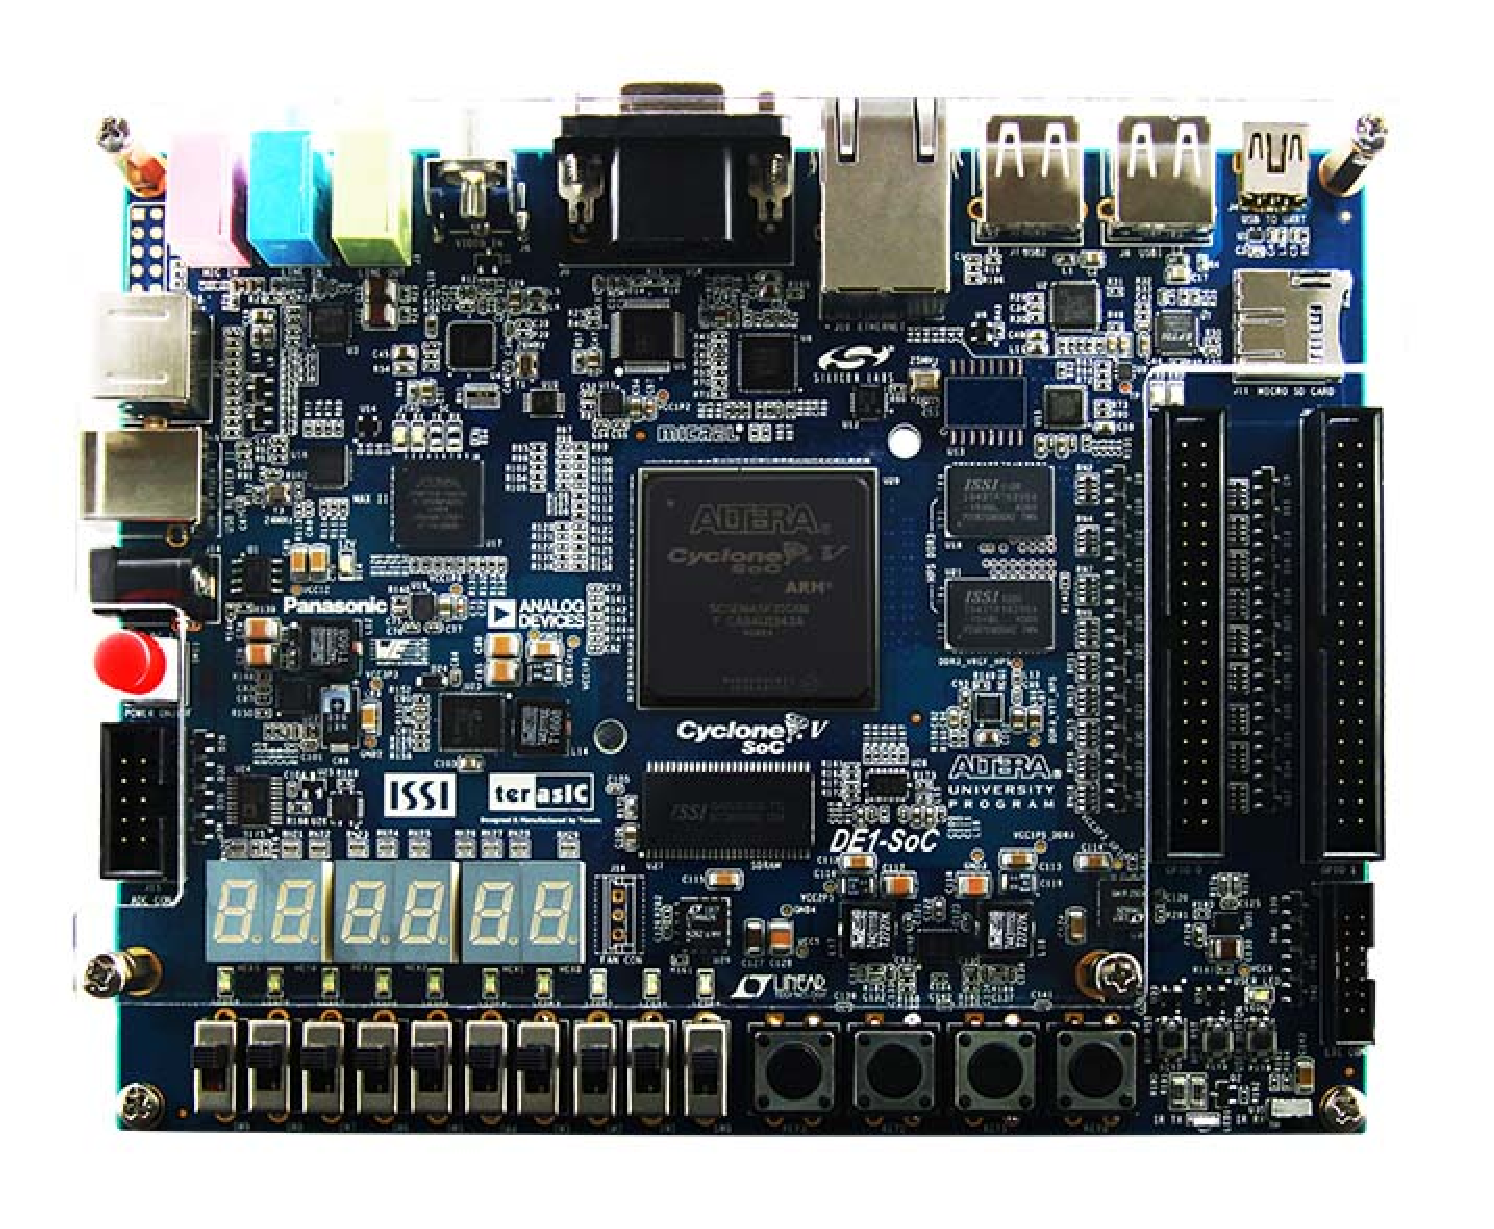
\includegraphics[scale=0.5]{DE1SoC.eps}
\vskip 0.1in
\end{center}

\begin{center}
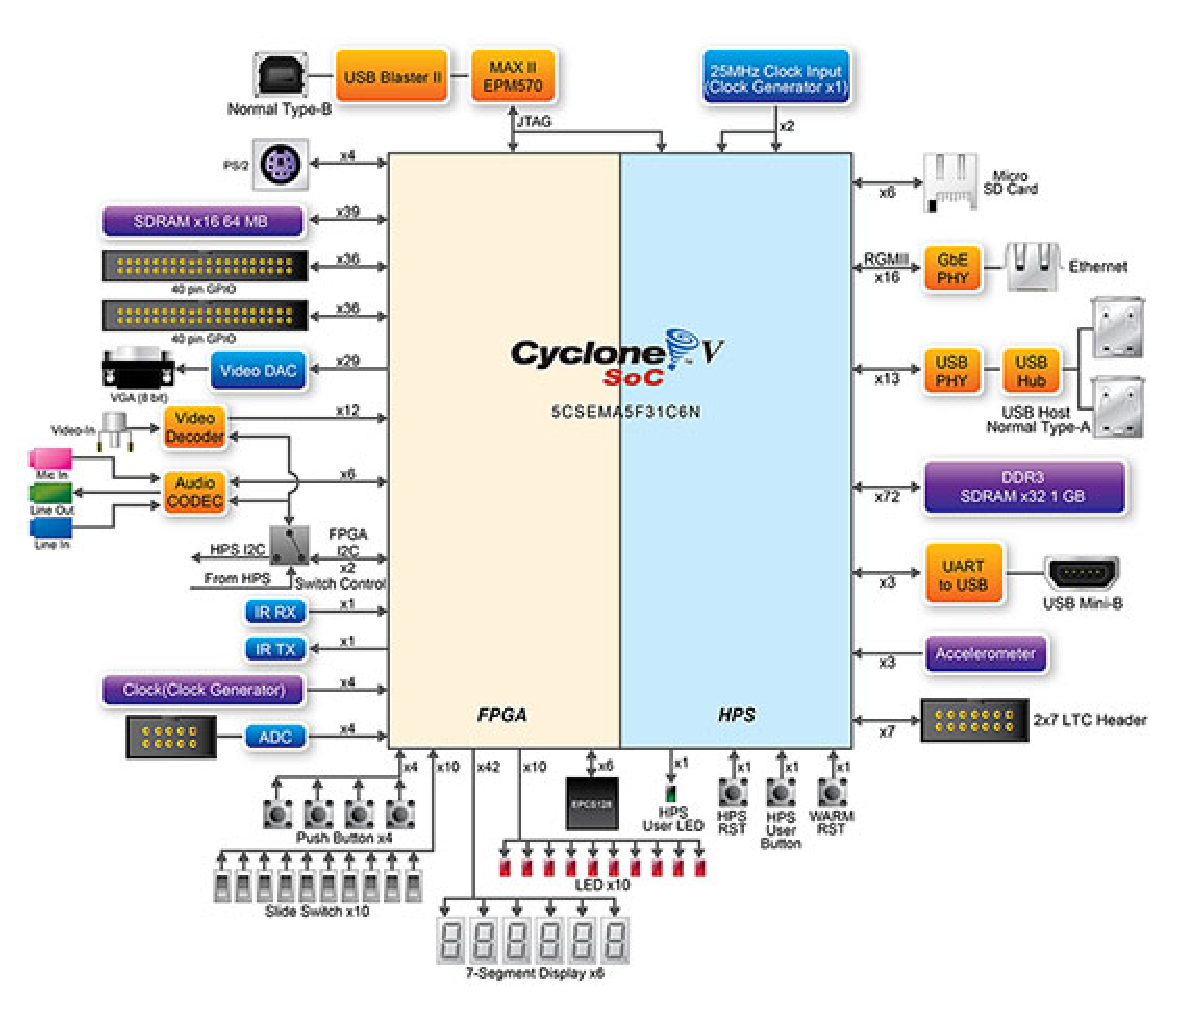
\includegraphics[scale=0.75]{DE1SoCports.eps}
\vskip 0.1in
\end{center}

\section{FPGA Background}
\begin{itemize}
\item {\bf First Use}
\url{http://wl.altera.com/customertraining/webex/Begin_Simple_FPGA_Design/presentation.html}
\end{itemize}

\subsection{Hardware Tradeoff Matrix\cite{4}}
\begin{tabular}{llllll}
         &x86&GPU&DSP&FPGA&$\mu{}$C\\
embed   &maybe &hard      &easy      &easy&easy\\
low power&unusual &nope  &sometimes &sometimes &yes\\
float op&good&excellent&excellent&possible&nope\\
int op&excellent&excellent&excellent&excellent&mediocore\\
control flow&excellent&challenging&air&challenging&excellent\\
io&mediocore&nope&ok&ginormous&ok\\
pipelining&nope&nope&nope&yes&nope\\
programmable&easy&medium&medius&challenging&easy\\
timing control&medium&what?&fair&excellent&fair\\
\end{tabular}

state machines / random numbers 
PSHDL / myHDL / Verilog / VHDL

Xilinx / Altera / Actel (microsem) / Lattice

Ethernet hardware chip
news.thomasnet.com/fullstory/hardwired-tcp-ip-ic-offloads-stack-for-high-speed-internet-490029

\subsection{FPGA Development Boards\cite{4}}
\begin{tabular}{llll}
& actel&altera&xilinx\\
cheap&PSHDL board&DE0-Nano&Papilo One (Spartan 3)\\
&&bemicro CV&mojo Vs (spartan 6)\\
&&&XuLA2-LX25\\
powerful&igloo 2 boards&cyclone 5/arria&artix/kintex/virtex\\
SoC&smartfusion2 starter kit&EBV SoCrates&MicroZedBoard\\
&SmartFusion Starter kit&&parallella\\
CPU+FPGA&Daenkrake&&Logi\\
\end{tabular}

deny by default

disaster recovery


stealing backups
recovery plan

software
  user-mode
  kernel-mode
  hypervisor
  firmware
  microcode
  hardware
  physics

hardware exfilt:
  http://es.slideshare.net/ortegaalfredo/deep-submicronbackdoorsortegasyscan2014slides
    modify chip to detect sequence
    toggle hardware line (e.g. led) to generate radio freq
    listen with radio

infilltration

size of information
  key is easy... use blinds
  database is hard ... large volume

cloud?

sysadmin attacks (snowden/anthem)

fpga/asic
runtime reconfigurable systems
\verb|http://media.ccc.de/browse/congress/2013/30C3_-_5443_-_en_-_saal_g_201312281830_-_introduction_to_processor_design_-_byterazor.html#video&t=370|
\verb|http://byterazor.federationhq.de/download/handout_30C3.pdf|

fpga 50 dollars
  serial cable
  logic analyzer
  VHDL / Verilog
\verb|http://tama-www.informatik.uni-hamburg.ed/vhdl/doc/cookbook/VHDL-Cookbook.pdf|

www.altera.com 6Gbps (starter kit)

regular, random machine audits (aka drug policy)
work from home?
Ring-level security policy?
finding out (e.g. watermarks, RFID tags)
dual computer policy? (plugged USB/secure only networking/loctite screws)

\begin{quote}
"Many businesses erro by putting too much faith in technology alone,
or by starting a security program with a technology blitz. The best
security technology in the world won't produce a good return on
investment without the foundation of security processes, policies, and
education. Instead, businesses should start by evaluating employee
behavior and the associated risks based on factors such as the locale
and the threat landscape. Then treat education, security training, and
business processes can be scuplted around that intelligence. At that
point, appropriate investments in security technology can be applied"
\cite{2}
\end{quote}

outsiders let inside
  "cleaner attacks"/"copier attacks"/"video stream encrypt"

BYOD
mobility
cloud
internet
wifi
USB
unauthorized software
email

provisioning
privileged account management
managing access

\section{DE1 gpio test}

\begin{verbatim}

GPIO1 is the GPIO connector nearest outside edge of board.
GPIO1 layout is (pin 1 is near USB port, on inside edge of connector)
   pin 1           pin 2
   pin 3           pin 4
   pin 5           pin 6
   pin 7           pin 8
   pin 9           pin 10
   pin 11 (VCC5V)  pin 12 (GND)
   pin 13          pin 14
   pin 15          pin 16
   pin 17          pin 18
   pin 19          pin 20
   pin 21          pin 22
   pin 23          pin 24
   pin 25          pin 26
   pin 27          pin 28
   pin 29 (VCC3.3) pin 30 (GND)
   pin 31          pin 32
   pin 33          pin 34
   pin 35          pin 36
   pin 37          pin 38
   pin 39          pin 40

Wire from GPIO1 pin 1 to LED-diode+ 
     from LED-diode- to 180ohm resistor
     from 180ohm resistor to GPIO1 pin 11 (VCC 5V)
Pushing KEY[0] should turn OFF this LED

Wire from GPIO1 pin 2 to LED-diode+ 
     from LED-diode- to 180ohm resistor
     from 180ohm resistor to GPIO1 pin 11 (VCC 5V)
Pushing KEY[1] should turn OFF this LED

Wire from GPIO1 pin 3 to LED-diode+ 
     from LED-diode- to 180ohm resistor
     from 180ohm resistor to GPIO1 pin 11 (VCC 5V)
Pushing KEY[2] should turn OFF this LED

Wire from GPIO1 pin 4 to LED-diode+ 
     from LED-diode- to 180ohm resistor
     from 180ohm resistor to GPIO1 pin 11 (VCC 5V)
Pushing KEY[3] should turn ON this LED

\end{verbatim}
\begin{verbatim}
library ieee;
use ieee.std_logic_1164.all;

ENTITY TPDblink IS 
 PORT (
  KEY: in std_logic_vector(3 downto 0);
  GPIO_1: out std_logic_vector(35 downto 0));
end ENTITY TPDblink;

architecture TPDblinkarch of TPDblink is
 begin 
  process(KEY)
   variable result: std_logic_vector(35 downto 0) 
       := "111111111111111111111111111111111111";
   begin 
	 if KEY(0)='1' THEN
     result(0) := '1';
	else 
	  result(0) := '0';
	end if;
	if KEY(1)='1' THEN
     result(1) := '1';
	else 
	  result(1) := '0';
	end if;
	if KEY(2)='1' THEN
     result(2) := '1';
	else 
	  result(2) := '0';
	end if;
	if KEY(3)='1' THEN
     result(3) := '0';
	else 
	  result(3) := '1';
	end if;
        GPIO_1 <= result;
  end process;
end architecture TPDblinkarch;
\end{verbatim}
\begin{verbatim}
#**************************************************************
# This .sdc file is created by Terasic Tool.
# Users are recommended to modify this file to match users logic.
#**************************************************************

#**************************************************************
# Create Clock
#**************************************************************
create_clock -period 20.000ns [get_ports CLOCK_50]
create_clock -period 20.000ns [get_ports CLOCK2_50]
create_clock -period 20.000ns [get_ports CLOCK3_50]
create_clock -period 20.000ns [get_ports CLOCK4_50]

# for enhancing USB BlasterII to be reliable, 25MHz
create_clock -name {altera_reserved_tck} -period 40 {altera_reserved_tck}
set_input_delay -clock altera_reserved_tck -clock_fall 3 [get_ports altera_reserved_tdi]
set_input_delay -clock altera_reserved_tck -clock_fall 3 [get_ports altera_reserved_tms]
set_output_delay -clock altera_reserved_tck 3 [get_ports altera_reserved_tdo]

#**************************************************************
# Create Generated Clock
#**************************************************************
derive_pll_clocks



#**************************************************************
# Set Clock Latency
#**************************************************************



#**************************************************************
# Set Clock Uncertainty
#**************************************************************
derive_clock_uncertainty



#**************************************************************
# Set Input Delay
#**************************************************************



#**************************************************************
# Set Output Delay
#**************************************************************



#**************************************************************
# Set Clock Groups
#**************************************************************



#**************************************************************
# Set False Path
#**************************************************************



#**************************************************************
# Set Multicycle Path
#**************************************************************



#**************************************************************
# Set Maximum Delay
#**************************************************************



#**************************************************************
# Set Minimum Delay
#**************************************************************



#**************************************************************
# Set Input Transition
#**************************************************************



#**************************************************************
# Set Load
#**************************************************************




\end{verbatim}
\begin{verbatim}
#============================================================
# Build by Terasic System Builder
#============================================================

set_global_assignment -name FAMILY "Cyclone V"
set_global_assignment -name DEVICE 5CSEMA5F31C6
set_global_assignment -name TOP_LEVEL_ENTITY "TPDblink"
set_global_assignment -name ORIGINAL_QUARTUS_VERSION 14.0
set_global_assignment -name LAST_QUARTUS_VERSION 14.1.0
set_global_assignment -name PROJECT_CREATION_TIME_DATE "21:01:14 FEBRUARY 27,2015"
set_global_assignment -name DEVICE_FILTER_PACKAGE FBGA
set_global_assignment -name DEVICE_FILTER_PIN_COUNT 896
set_global_assignment -name DEVICE_FILTER_SPEED_GRADE 6

#============================================================
# ADC
#============================================================
set_location_assignment PIN_AJ4 -to ADC_CS_N
set_instance_assignment -name IO_STANDARD "3.3-V LVTTL" -to ADC_CS_N
set_location_assignment PIN_AK4 -to ADC_DIN
set_instance_assignment -name IO_STANDARD "3.3-V LVTTL" -to ADC_DIN
set_location_assignment PIN_AK3 -to ADC_DOUT
set_instance_assignment -name IO_STANDARD "3.3-V LVTTL" -to ADC_DOUT
set_location_assignment PIN_AK2 -to ADC_SCLK
set_instance_assignment -name IO_STANDARD "3.3-V LVTTL" -to ADC_SCLK

#============================================================
# Audio
#============================================================
set_location_assignment PIN_K7 -to AUD_ADCDAT
set_instance_assignment -name IO_STANDARD "3.3-V LVTTL" -to AUD_ADCDAT
set_location_assignment PIN_K8 -to AUD_ADCLRCK
set_instance_assignment -name IO_STANDARD "3.3-V LVTTL" -to AUD_ADCLRCK
set_location_assignment PIN_H7 -to AUD_BCLK
set_instance_assignment -name IO_STANDARD "3.3-V LVTTL" -to AUD_BCLK
set_location_assignment PIN_J7 -to AUD_DACDAT
set_instance_assignment -name IO_STANDARD "3.3-V LVTTL" -to AUD_DACDAT
set_location_assignment PIN_H8 -to AUD_DACLRCK
set_instance_assignment -name IO_STANDARD "3.3-V LVTTL" -to AUD_DACLRCK
set_location_assignment PIN_G7 -to AUD_XCK
set_instance_assignment -name IO_STANDARD "3.3-V LVTTL" -to AUD_XCK

#============================================================
# CLOCK
#============================================================
set_location_assignment PIN_AF14 -to CLOCK_50
set_instance_assignment -name IO_STANDARD "3.3-V LVTTL" -to CLOCK_50
set_location_assignment PIN_AA16 -to CLOCK2_50
set_instance_assignment -name IO_STANDARD "3.3-V LVTTL" -to CLOCK2_50
set_location_assignment PIN_Y26 -to CLOCK3_50
set_instance_assignment -name IO_STANDARD "3.3-V LVTTL" -to CLOCK3_50
set_location_assignment PIN_K14 -to CLOCK4_50
set_instance_assignment -name IO_STANDARD "3.3-V LVTTL" -to CLOCK4_50

#============================================================
# SDRAM
#============================================================
set_location_assignment PIN_AK14 -to DRAM_ADDR[0]
set_instance_assignment -name IO_STANDARD "3.3-V LVTTL" -to DRAM_ADDR[0]
set_location_assignment PIN_AH14 -to DRAM_ADDR[1]
set_instance_assignment -name IO_STANDARD "3.3-V LVTTL" -to DRAM_ADDR[1]
set_location_assignment PIN_AG15 -to DRAM_ADDR[2]
set_instance_assignment -name IO_STANDARD "3.3-V LVTTL" -to DRAM_ADDR[2]
set_location_assignment PIN_AE14 -to DRAM_ADDR[3]
set_instance_assignment -name IO_STANDARD "3.3-V LVTTL" -to DRAM_ADDR[3]
set_location_assignment PIN_AB15 -to DRAM_ADDR[4]
set_instance_assignment -name IO_STANDARD "3.3-V LVTTL" -to DRAM_ADDR[4]
set_location_assignment PIN_AC14 -to DRAM_ADDR[5]
set_instance_assignment -name IO_STANDARD "3.3-V LVTTL" -to DRAM_ADDR[5]
set_location_assignment PIN_AD14 -to DRAM_ADDR[6]
set_instance_assignment -name IO_STANDARD "3.3-V LVTTL" -to DRAM_ADDR[6]
set_location_assignment PIN_AF15 -to DRAM_ADDR[7]
set_instance_assignment -name IO_STANDARD "3.3-V LVTTL" -to DRAM_ADDR[7]
set_location_assignment PIN_AH15 -to DRAM_ADDR[8]
set_instance_assignment -name IO_STANDARD "3.3-V LVTTL" -to DRAM_ADDR[8]
set_location_assignment PIN_AG13 -to DRAM_ADDR[9]
set_instance_assignment -name IO_STANDARD "3.3-V LVTTL" -to DRAM_ADDR[9]
set_location_assignment PIN_AG12 -to DRAM_ADDR[10]
set_instance_assignment -name IO_STANDARD "3.3-V LVTTL" -to DRAM_ADDR[10]
set_location_assignment PIN_AH13 -to DRAM_ADDR[11]
set_instance_assignment -name IO_STANDARD "3.3-V LVTTL" -to DRAM_ADDR[11]
set_location_assignment PIN_AJ14 -to DRAM_ADDR[12]
set_instance_assignment -name IO_STANDARD "3.3-V LVTTL" -to DRAM_ADDR[12]
set_location_assignment PIN_AF13 -to DRAM_BA[0]
set_instance_assignment -name IO_STANDARD "3.3-V LVTTL" -to DRAM_BA[0]
set_location_assignment PIN_AJ12 -to DRAM_BA[1]
set_instance_assignment -name IO_STANDARD "3.3-V LVTTL" -to DRAM_BA[1]
set_location_assignment PIN_AF11 -to DRAM_CAS_N
set_instance_assignment -name IO_STANDARD "3.3-V LVTTL" -to DRAM_CAS_N
set_location_assignment PIN_AK13 -to DRAM_CKE
set_instance_assignment -name IO_STANDARD "3.3-V LVTTL" -to DRAM_CKE
set_location_assignment PIN_AG11 -to DRAM_CS_N
set_instance_assignment -name IO_STANDARD "3.3-V LVTTL" -to DRAM_CS_N
set_location_assignment PIN_AH12 -to DRAM_CLK
set_instance_assignment -name IO_STANDARD "3.3-V LVTTL" -to DRAM_CLK
set_location_assignment PIN_AK6 -to DRAM_DQ[0]
set_instance_assignment -name IO_STANDARD "3.3-V LVTTL" -to DRAM_DQ[0]
set_location_assignment PIN_AJ7 -to DRAM_DQ[1]
set_instance_assignment -name IO_STANDARD "3.3-V LVTTL" -to DRAM_DQ[1]
set_location_assignment PIN_AK7 -to DRAM_DQ[2]
set_instance_assignment -name IO_STANDARD "3.3-V LVTTL" -to DRAM_DQ[2]
set_location_assignment PIN_AK8 -to DRAM_DQ[3]
set_instance_assignment -name IO_STANDARD "3.3-V LVTTL" -to DRAM_DQ[3]
set_location_assignment PIN_AK9 -to DRAM_DQ[4]
set_instance_assignment -name IO_STANDARD "3.3-V LVTTL" -to DRAM_DQ[4]
set_location_assignment PIN_AG10 -to DRAM_DQ[5]
set_instance_assignment -name IO_STANDARD "3.3-V LVTTL" -to DRAM_DQ[5]
set_location_assignment PIN_AK11 -to DRAM_DQ[6]
set_instance_assignment -name IO_STANDARD "3.3-V LVTTL" -to DRAM_DQ[6]
set_location_assignment PIN_AJ11 -to DRAM_DQ[7]
set_instance_assignment -name IO_STANDARD "3.3-V LVTTL" -to DRAM_DQ[7]
set_location_assignment PIN_AH10 -to DRAM_DQ[8]
set_instance_assignment -name IO_STANDARD "3.3-V LVTTL" -to DRAM_DQ[8]
set_location_assignment PIN_AJ10 -to DRAM_DQ[9]
set_instance_assignment -name IO_STANDARD "3.3-V LVTTL" -to DRAM_DQ[9]
set_location_assignment PIN_AJ9 -to DRAM_DQ[10]
set_instance_assignment -name IO_STANDARD "3.3-V LVTTL" -to DRAM_DQ[10]
set_location_assignment PIN_AH9 -to DRAM_DQ[11]
set_instance_assignment -name IO_STANDARD "3.3-V LVTTL" -to DRAM_DQ[11]
set_location_assignment PIN_AH8 -to DRAM_DQ[12]
set_instance_assignment -name IO_STANDARD "3.3-V LVTTL" -to DRAM_DQ[12]
set_location_assignment PIN_AH7 -to DRAM_DQ[13]
set_instance_assignment -name IO_STANDARD "3.3-V LVTTL" -to DRAM_DQ[13]
set_location_assignment PIN_AJ6 -to DRAM_DQ[14]
set_instance_assignment -name IO_STANDARD "3.3-V LVTTL" -to DRAM_DQ[14]
set_location_assignment PIN_AJ5 -to DRAM_DQ[15]
set_instance_assignment -name IO_STANDARD "3.3-V LVTTL" -to DRAM_DQ[15]
set_location_assignment PIN_AB13 -to DRAM_LDQM
set_instance_assignment -name IO_STANDARD "3.3-V LVTTL" -to DRAM_LDQM
set_location_assignment PIN_AE13 -to DRAM_RAS_N
set_instance_assignment -name IO_STANDARD "3.3-V LVTTL" -to DRAM_RAS_N
set_location_assignment PIN_AK12 -to DRAM_UDQM
set_instance_assignment -name IO_STANDARD "3.3-V LVTTL" -to DRAM_UDQM
set_location_assignment PIN_AA13 -to DRAM_WE_N
set_instance_assignment -name IO_STANDARD "3.3-V LVTTL" -to DRAM_WE_N

#============================================================
# I2C for Audio and Video-In
#============================================================
set_location_assignment PIN_J12 -to FPGA_I2C_SCLK
set_instance_assignment -name IO_STANDARD "3.3-V LVTTL" -to FPGA_I2C_SCLK
set_location_assignment PIN_K12 -to FPGA_I2C_SDAT
set_instance_assignment -name IO_STANDARD "3.3-V LVTTL" -to FPGA_I2C_SDAT

#============================================================
# SEG7
#============================================================
set_location_assignment PIN_AE26 -to HEX0[0]
set_instance_assignment -name IO_STANDARD "3.3-V LVTTL" -to HEX0[0]
set_location_assignment PIN_AE27 -to HEX0[1]
set_instance_assignment -name IO_STANDARD "3.3-V LVTTL" -to HEX0[1]
set_location_assignment PIN_AE28 -to HEX0[2]
set_instance_assignment -name IO_STANDARD "3.3-V LVTTL" -to HEX0[2]
set_location_assignment PIN_AG27 -to HEX0[3]
set_instance_assignment -name IO_STANDARD "3.3-V LVTTL" -to HEX0[3]
set_location_assignment PIN_AF28 -to HEX0[4]
set_instance_assignment -name IO_STANDARD "3.3-V LVTTL" -to HEX0[4]
set_location_assignment PIN_AG28 -to HEX0[5]
set_instance_assignment -name IO_STANDARD "3.3-V LVTTL" -to HEX0[5]
set_location_assignment PIN_AH28 -to HEX0[6]
set_instance_assignment -name IO_STANDARD "3.3-V LVTTL" -to HEX0[6]
set_location_assignment PIN_AJ29 -to HEX1[0]
set_instance_assignment -name IO_STANDARD "3.3-V LVTTL" -to HEX1[0]
set_location_assignment PIN_AH29 -to HEX1[1]
set_instance_assignment -name IO_STANDARD "3.3-V LVTTL" -to HEX1[1]
set_location_assignment PIN_AH30 -to HEX1[2]
set_instance_assignment -name IO_STANDARD "3.3-V LVTTL" -to HEX1[2]
set_location_assignment PIN_AG30 -to HEX1[3]
set_instance_assignment -name IO_STANDARD "3.3-V LVTTL" -to HEX1[3]
set_location_assignment PIN_AF29 -to HEX1[4]
set_instance_assignment -name IO_STANDARD "3.3-V LVTTL" -to HEX1[4]
set_location_assignment PIN_AF30 -to HEX1[5]
set_instance_assignment -name IO_STANDARD "3.3-V LVTTL" -to HEX1[5]
set_location_assignment PIN_AD27 -to HEX1[6]
set_instance_assignment -name IO_STANDARD "3.3-V LVTTL" -to HEX1[6]
set_location_assignment PIN_AB23 -to HEX2[0]
set_instance_assignment -name IO_STANDARD "3.3-V LVTTL" -to HEX2[0]
set_location_assignment PIN_AE29 -to HEX2[1]
set_instance_assignment -name IO_STANDARD "3.3-V LVTTL" -to HEX2[1]
set_location_assignment PIN_AD29 -to HEX2[2]
set_instance_assignment -name IO_STANDARD "3.3-V LVTTL" -to HEX2[2]
set_location_assignment PIN_AC28 -to HEX2[3]
set_instance_assignment -name IO_STANDARD "3.3-V LVTTL" -to HEX2[3]
set_location_assignment PIN_AD30 -to HEX2[4]
set_instance_assignment -name IO_STANDARD "3.3-V LVTTL" -to HEX2[4]
set_location_assignment PIN_AC29 -to HEX2[5]
set_instance_assignment -name IO_STANDARD "3.3-V LVTTL" -to HEX2[5]
set_location_assignment PIN_AC30 -to HEX2[6]
set_instance_assignment -name IO_STANDARD "3.3-V LVTTL" -to HEX2[6]
set_location_assignment PIN_AD26 -to HEX3[0]
set_instance_assignment -name IO_STANDARD "3.3-V LVTTL" -to HEX3[0]
set_location_assignment PIN_AC27 -to HEX3[1]
set_instance_assignment -name IO_STANDARD "3.3-V LVTTL" -to HEX3[1]
set_location_assignment PIN_AD25 -to HEX3[2]
set_instance_assignment -name IO_STANDARD "3.3-V LVTTL" -to HEX3[2]
set_location_assignment PIN_AC25 -to HEX3[3]
set_instance_assignment -name IO_STANDARD "3.3-V LVTTL" -to HEX3[3]
set_location_assignment PIN_AB28 -to HEX3[4]
set_instance_assignment -name IO_STANDARD "3.3-V LVTTL" -to HEX3[4]
set_location_assignment PIN_AB25 -to HEX3[5]
set_instance_assignment -name IO_STANDARD "3.3-V LVTTL" -to HEX3[5]
set_location_assignment PIN_AB22 -to HEX3[6]
set_instance_assignment -name IO_STANDARD "3.3-V LVTTL" -to HEX3[6]
set_location_assignment PIN_AA24 -to HEX4[0]
set_instance_assignment -name IO_STANDARD "3.3-V LVTTL" -to HEX4[0]
set_location_assignment PIN_Y23 -to HEX4[1]
set_instance_assignment -name IO_STANDARD "3.3-V LVTTL" -to HEX4[1]
set_location_assignment PIN_Y24 -to HEX4[2]
set_instance_assignment -name IO_STANDARD "3.3-V LVTTL" -to HEX4[2]
set_location_assignment PIN_W22 -to HEX4[3]
set_instance_assignment -name IO_STANDARD "3.3-V LVTTL" -to HEX4[3]
set_location_assignment PIN_W24 -to HEX4[4]
set_instance_assignment -name IO_STANDARD "3.3-V LVTTL" -to HEX4[4]
set_location_assignment PIN_V23 -to HEX4[5]
set_instance_assignment -name IO_STANDARD "3.3-V LVTTL" -to HEX4[5]
set_location_assignment PIN_W25 -to HEX4[6]
set_instance_assignment -name IO_STANDARD "3.3-V LVTTL" -to HEX4[6]
set_location_assignment PIN_V25 -to HEX5[0]
set_instance_assignment -name IO_STANDARD "3.3-V LVTTL" -to HEX5[0]
set_location_assignment PIN_AA28 -to HEX5[1]
set_instance_assignment -name IO_STANDARD "3.3-V LVTTL" -to HEX5[1]
set_location_assignment PIN_Y27 -to HEX5[2]
set_instance_assignment -name IO_STANDARD "3.3-V LVTTL" -to HEX5[2]
set_location_assignment PIN_AB27 -to HEX5[3]
set_instance_assignment -name IO_STANDARD "3.3-V LVTTL" -to HEX5[3]
set_location_assignment PIN_AB26 -to HEX5[4]
set_instance_assignment -name IO_STANDARD "3.3-V LVTTL" -to HEX5[4]
set_location_assignment PIN_AA26 -to HEX5[5]
set_instance_assignment -name IO_STANDARD "3.3-V LVTTL" -to HEX5[5]
set_location_assignment PIN_AA25 -to HEX5[6]
set_instance_assignment -name IO_STANDARD "3.3-V LVTTL" -to HEX5[6]

#============================================================
# IR
#============================================================
set_location_assignment PIN_AA30 -to IRDA_RXD
set_instance_assignment -name IO_STANDARD "3.3-V LVTTL" -to IRDA_RXD
set_location_assignment PIN_AB30 -to IRDA_TXD
set_instance_assignment -name IO_STANDARD "3.3-V LVTTL" -to IRDA_TXD

#============================================================
# KEY
#============================================================
set_location_assignment PIN_AA14 -to KEY[0]
set_instance_assignment -name IO_STANDARD "3.3-V LVTTL" -to KEY[0]
set_location_assignment PIN_AA15 -to KEY[1]
set_instance_assignment -name IO_STANDARD "3.3-V LVTTL" -to KEY[1]
set_location_assignment PIN_W15 -to KEY[2]
set_instance_assignment -name IO_STANDARD "3.3-V LVTTL" -to KEY[2]
set_location_assignment PIN_Y16 -to KEY[3]
set_instance_assignment -name IO_STANDARD "3.3-V LVTTL" -to KEY[3]

#============================================================
# LED
#============================================================
set_location_assignment PIN_V16 -to LEDR[0]
set_instance_assignment -name IO_STANDARD "3.3-V LVTTL" -to LEDR[0]
set_location_assignment PIN_W16 -to LEDR[1]
set_instance_assignment -name IO_STANDARD "3.3-V LVTTL" -to LEDR[1]
set_location_assignment PIN_V17 -to LEDR[2]
set_instance_assignment -name IO_STANDARD "3.3-V LVTTL" -to LEDR[2]
set_location_assignment PIN_V18 -to LEDR[3]
set_instance_assignment -name IO_STANDARD "3.3-V LVTTL" -to LEDR[3]
set_location_assignment PIN_W17 -to LEDR[4]
set_instance_assignment -name IO_STANDARD "3.3-V LVTTL" -to LEDR[4]
set_location_assignment PIN_W19 -to LEDR[5]
set_instance_assignment -name IO_STANDARD "3.3-V LVTTL" -to LEDR[5]
set_location_assignment PIN_Y19 -to LEDR[6]
set_instance_assignment -name IO_STANDARD "3.3-V LVTTL" -to LEDR[6]
set_location_assignment PIN_W20 -to LEDR[7]
set_instance_assignment -name IO_STANDARD "3.3-V LVTTL" -to LEDR[7]
set_location_assignment PIN_W21 -to LEDR[8]
set_instance_assignment -name IO_STANDARD "3.3-V LVTTL" -to LEDR[8]
set_location_assignment PIN_Y21 -to LEDR[9]
set_instance_assignment -name IO_STANDARD "3.3-V LVTTL" -to LEDR[9]

#============================================================
# PS2
#============================================================
set_location_assignment PIN_AD7 -to PS2_CLK
set_instance_assignment -name IO_STANDARD "3.3-V LVTTL" -to PS2_CLK
set_location_assignment PIN_AD9 -to PS2_CLK2
set_instance_assignment -name IO_STANDARD "3.3-V LVTTL" -to PS2_CLK2
set_location_assignment PIN_AE7 -to PS2_DAT
set_instance_assignment -name IO_STANDARD "3.3-V LVTTL" -to PS2_DAT
set_location_assignment PIN_AE9 -to PS2_DAT2
set_instance_assignment -name IO_STANDARD "3.3-V LVTTL" -to PS2_DAT2

#============================================================
# SW
#============================================================
set_location_assignment PIN_AB12 -to SW[0]
set_instance_assignment -name IO_STANDARD "3.3-V LVTTL" -to SW[0]
set_location_assignment PIN_AC12 -to SW[1]
set_instance_assignment -name IO_STANDARD "3.3-V LVTTL" -to SW[1]
set_location_assignment PIN_AF9 -to SW[2]
set_instance_assignment -name IO_STANDARD "3.3-V LVTTL" -to SW[2]
set_location_assignment PIN_AF10 -to SW[3]
set_instance_assignment -name IO_STANDARD "3.3-V LVTTL" -to SW[3]
set_location_assignment PIN_AD11 -to SW[4]
set_instance_assignment -name IO_STANDARD "3.3-V LVTTL" -to SW[4]
set_location_assignment PIN_AD12 -to SW[5]
set_instance_assignment -name IO_STANDARD "3.3-V LVTTL" -to SW[5]
set_location_assignment PIN_AE11 -to SW[6]
set_instance_assignment -name IO_STANDARD "3.3-V LVTTL" -to SW[6]
set_location_assignment PIN_AC9 -to SW[7]
set_instance_assignment -name IO_STANDARD "3.3-V LVTTL" -to SW[7]
set_location_assignment PIN_AD10 -to SW[8]
set_instance_assignment -name IO_STANDARD "3.3-V LVTTL" -to SW[8]
set_location_assignment PIN_AE12 -to SW[9]
set_instance_assignment -name IO_STANDARD "3.3-V LVTTL" -to SW[9]

#============================================================
# Video-In
#============================================================
set_location_assignment PIN_H15 -to TD_CLK27
set_instance_assignment -name IO_STANDARD "3.3-V LVTTL" -to TD_CLK27
set_location_assignment PIN_D2 -to TD_DATA[0]
set_instance_assignment -name IO_STANDARD "3.3-V LVTTL" -to TD_DATA[0]
set_location_assignment PIN_B1 -to TD_DATA[1]
set_instance_assignment -name IO_STANDARD "3.3-V LVTTL" -to TD_DATA[1]
set_location_assignment PIN_E2 -to TD_DATA[2]
set_instance_assignment -name IO_STANDARD "3.3-V LVTTL" -to TD_DATA[2]
set_location_assignment PIN_B2 -to TD_DATA[3]
set_instance_assignment -name IO_STANDARD "3.3-V LVTTL" -to TD_DATA[3]
set_location_assignment PIN_D1 -to TD_DATA[4]
set_instance_assignment -name IO_STANDARD "3.3-V LVTTL" -to TD_DATA[4]
set_location_assignment PIN_E1 -to TD_DATA[5]
set_instance_assignment -name IO_STANDARD "3.3-V LVTTL" -to TD_DATA[5]
set_location_assignment PIN_C2 -to TD_DATA[6]
set_instance_assignment -name IO_STANDARD "3.3-V LVTTL" -to TD_DATA[6]
set_location_assignment PIN_B3 -to TD_DATA[7]
set_instance_assignment -name IO_STANDARD "3.3-V LVTTL" -to TD_DATA[7]
set_location_assignment PIN_A5 -to TD_HS
set_instance_assignment -name IO_STANDARD "3.3-V LVTTL" -to TD_HS
set_location_assignment PIN_F6 -to TD_RESET_N
set_instance_assignment -name IO_STANDARD "3.3-V LVTTL" -to TD_RESET_N
set_location_assignment PIN_A3 -to TD_VS
set_instance_assignment -name IO_STANDARD "3.3-V LVTTL" -to TD_VS

#============================================================
# VGA
#============================================================
set_location_assignment PIN_B13 -to VGA_B[0]
set_instance_assignment -name IO_STANDARD "3.3-V LVTTL" -to VGA_B[0]
set_location_assignment PIN_G13 -to VGA_B[1]
set_instance_assignment -name IO_STANDARD "3.3-V LVTTL" -to VGA_B[1]
set_location_assignment PIN_H13 -to VGA_B[2]
set_instance_assignment -name IO_STANDARD "3.3-V LVTTL" -to VGA_B[2]
set_location_assignment PIN_F14 -to VGA_B[3]
set_instance_assignment -name IO_STANDARD "3.3-V LVTTL" -to VGA_B[3]
set_location_assignment PIN_H14 -to VGA_B[4]
set_instance_assignment -name IO_STANDARD "3.3-V LVTTL" -to VGA_B[4]
set_location_assignment PIN_F15 -to VGA_B[5]
set_instance_assignment -name IO_STANDARD "3.3-V LVTTL" -to VGA_B[5]
set_location_assignment PIN_G15 -to VGA_B[6]
set_instance_assignment -name IO_STANDARD "3.3-V LVTTL" -to VGA_B[6]
set_location_assignment PIN_J14 -to VGA_B[7]
set_instance_assignment -name IO_STANDARD "3.3-V LVTTL" -to VGA_B[7]
set_location_assignment PIN_F10 -to VGA_BLANK_N
set_instance_assignment -name IO_STANDARD "3.3-V LVTTL" -to VGA_BLANK_N
set_location_assignment PIN_A11 -to VGA_CLK
set_instance_assignment -name IO_STANDARD "3.3-V LVTTL" -to VGA_CLK
set_location_assignment PIN_J9 -to VGA_G[0]
set_instance_assignment -name IO_STANDARD "3.3-V LVTTL" -to VGA_G[0]
set_location_assignment PIN_J10 -to VGA_G[1]
set_instance_assignment -name IO_STANDARD "3.3-V LVTTL" -to VGA_G[1]
set_location_assignment PIN_H12 -to VGA_G[2]
set_instance_assignment -name IO_STANDARD "3.3-V LVTTL" -to VGA_G[2]
set_location_assignment PIN_G10 -to VGA_G[3]
set_instance_assignment -name IO_STANDARD "3.3-V LVTTL" -to VGA_G[3]
set_location_assignment PIN_G11 -to VGA_G[4]
set_instance_assignment -name IO_STANDARD "3.3-V LVTTL" -to VGA_G[4]
set_location_assignment PIN_G12 -to VGA_G[5]
set_instance_assignment -name IO_STANDARD "3.3-V LVTTL" -to VGA_G[5]
set_location_assignment PIN_F11 -to VGA_G[6]
set_instance_assignment -name IO_STANDARD "3.3-V LVTTL" -to VGA_G[6]
set_location_assignment PIN_E11 -to VGA_G[7]
set_instance_assignment -name IO_STANDARD "3.3-V LVTTL" -to VGA_G[7]
set_location_assignment PIN_B11 -to VGA_HS
set_instance_assignment -name IO_STANDARD "3.3-V LVTTL" -to VGA_HS
set_location_assignment PIN_A13 -to VGA_R[0]
set_instance_assignment -name IO_STANDARD "3.3-V LVTTL" -to VGA_R[0]
set_location_assignment PIN_C13 -to VGA_R[1]
set_instance_assignment -name IO_STANDARD "3.3-V LVTTL" -to VGA_R[1]
set_location_assignment PIN_E13 -to VGA_R[2]
set_instance_assignment -name IO_STANDARD "3.3-V LVTTL" -to VGA_R[2]
set_location_assignment PIN_B12 -to VGA_R[3]
set_instance_assignment -name IO_STANDARD "3.3-V LVTTL" -to VGA_R[3]
set_location_assignment PIN_C12 -to VGA_R[4]
set_instance_assignment -name IO_STANDARD "3.3-V LVTTL" -to VGA_R[4]
set_location_assignment PIN_D12 -to VGA_R[5]
set_instance_assignment -name IO_STANDARD "3.3-V LVTTL" -to VGA_R[5]
set_location_assignment PIN_E12 -to VGA_R[6]
set_instance_assignment -name IO_STANDARD "3.3-V LVTTL" -to VGA_R[6]
set_location_assignment PIN_F13 -to VGA_R[7]
set_instance_assignment -name IO_STANDARD "3.3-V LVTTL" -to VGA_R[7]
set_location_assignment PIN_C10 -to VGA_SYNC_N
set_instance_assignment -name IO_STANDARD "3.3-V LVTTL" -to VGA_SYNC_N
set_location_assignment PIN_D11 -to VGA_VS
set_instance_assignment -name IO_STANDARD "3.3-V LVTTL" -to VGA_VS

#============================================================
# HPS
#============================================================
set_instance_assignment -name IO_STANDARD "SSTL-15 CLASS I" -to HPS_DDR3_ADDR[0]
set_instance_assignment -name IO_STANDARD "SSTL-15 CLASS I" -to HPS_DDR3_ADDR[1]
set_instance_assignment -name IO_STANDARD "SSTL-15 CLASS I" -to HPS_DDR3_ADDR[2]
set_instance_assignment -name IO_STANDARD "SSTL-15 CLASS I" -to HPS_DDR3_ADDR[3]
set_instance_assignment -name IO_STANDARD "SSTL-15 CLASS I" -to HPS_DDR3_ADDR[4]
set_instance_assignment -name IO_STANDARD "SSTL-15 CLASS I" -to HPS_DDR3_ADDR[5]
set_instance_assignment -name IO_STANDARD "SSTL-15 CLASS I" -to HPS_DDR3_ADDR[6]
set_instance_assignment -name IO_STANDARD "SSTL-15 CLASS I" -to HPS_DDR3_ADDR[7]
set_instance_assignment -name IO_STANDARD "SSTL-15 CLASS I" -to HPS_DDR3_ADDR[8]
set_instance_assignment -name IO_STANDARD "SSTL-15 CLASS I" -to HPS_DDR3_ADDR[9]
set_instance_assignment -name IO_STANDARD "SSTL-15 CLASS I" -to HPS_DDR3_ADDR[10]
set_instance_assignment -name IO_STANDARD "SSTL-15 CLASS I" -to HPS_DDR3_ADDR[11]
set_instance_assignment -name IO_STANDARD "SSTL-15 CLASS I" -to HPS_DDR3_ADDR[12]
set_instance_assignment -name IO_STANDARD "SSTL-15 CLASS I" -to HPS_DDR3_ADDR[13]
set_instance_assignment -name IO_STANDARD "SSTL-15 CLASS I" -to HPS_DDR3_ADDR[14]
set_instance_assignment -name IO_STANDARD "SSTL-15 CLASS I" -to HPS_DDR3_BA[0]
set_instance_assignment -name IO_STANDARD "SSTL-15 CLASS I" -to HPS_DDR3_BA[1]
set_instance_assignment -name IO_STANDARD "SSTL-15 CLASS I" -to HPS_DDR3_BA[2]
set_instance_assignment -name IO_STANDARD "SSTL-15 CLASS I" -to HPS_DDR3_DM[0]
set_instance_assignment -name IO_STANDARD "SSTL-15 CLASS I" -to HPS_DDR3_DM[1]
set_instance_assignment -name IO_STANDARD "SSTL-15 CLASS I" -to HPS_DDR3_DM[2]
set_instance_assignment -name IO_STANDARD "SSTL-15 CLASS I" -to HPS_DDR3_DM[3]
set_instance_assignment -name IO_STANDARD "SSTL-15 CLASS I" -to HPS_DDR3_DQ[0]
set_instance_assignment -name IO_STANDARD "SSTL-15 CLASS I" -to HPS_DDR3_DQ[1]
set_instance_assignment -name IO_STANDARD "SSTL-15 CLASS I" -to HPS_DDR3_DQ[2]
set_instance_assignment -name IO_STANDARD "SSTL-15 CLASS I" -to HPS_DDR3_DQ[3]
set_instance_assignment -name IO_STANDARD "SSTL-15 CLASS I" -to HPS_DDR3_DQ[4]
set_instance_assignment -name IO_STANDARD "SSTL-15 CLASS I" -to HPS_DDR3_DQ[5]
set_instance_assignment -name IO_STANDARD "SSTL-15 CLASS I" -to HPS_DDR3_DQ[6]
set_instance_assignment -name IO_STANDARD "SSTL-15 CLASS I" -to HPS_DDR3_DQ[7]
set_instance_assignment -name IO_STANDARD "SSTL-15 CLASS I" -to HPS_DDR3_DQ[8]
set_instance_assignment -name IO_STANDARD "SSTL-15 CLASS I" -to HPS_DDR3_DQ[9]
set_instance_assignment -name IO_STANDARD "SSTL-15 CLASS I" -to HPS_DDR3_DQ[10]
set_instance_assignment -name IO_STANDARD "SSTL-15 CLASS I" -to HPS_DDR3_DQ[11]
set_instance_assignment -name IO_STANDARD "SSTL-15 CLASS I" -to HPS_DDR3_DQ[12]
set_instance_assignment -name IO_STANDARD "SSTL-15 CLASS I" -to HPS_DDR3_DQ[13]
set_instance_assignment -name IO_STANDARD "SSTL-15 CLASS I" -to HPS_DDR3_DQ[14]
set_instance_assignment -name IO_STANDARD "SSTL-15 CLASS I" -to HPS_DDR3_DQ[15]
set_instance_assignment -name IO_STANDARD "SSTL-15 CLASS I" -to HPS_DDR3_DQ[16]
set_instance_assignment -name IO_STANDARD "SSTL-15 CLASS I" -to HPS_DDR3_DQ[17]
set_instance_assignment -name IO_STANDARD "SSTL-15 CLASS I" -to HPS_DDR3_DQ[18]
set_instance_assignment -name IO_STANDARD "SSTL-15 CLASS I" -to HPS_DDR3_DQ[19]
set_instance_assignment -name IO_STANDARD "SSTL-15 CLASS I" -to HPS_DDR3_DQ[20]
set_instance_assignment -name IO_STANDARD "SSTL-15 CLASS I" -to HPS_DDR3_DQ[21]
set_instance_assignment -name IO_STANDARD "SSTL-15 CLASS I" -to HPS_DDR3_DQ[22]
set_instance_assignment -name IO_STANDARD "SSTL-15 CLASS I" -to HPS_DDR3_DQ[23]
set_instance_assignment -name IO_STANDARD "SSTL-15 CLASS I" -to HPS_DDR3_DQ[24]
set_instance_assignment -name IO_STANDARD "SSTL-15 CLASS I" -to HPS_DDR3_DQ[25]
set_instance_assignment -name IO_STANDARD "SSTL-15 CLASS I" -to HPS_DDR3_DQ[26]
set_instance_assignment -name IO_STANDARD "SSTL-15 CLASS I" -to HPS_DDR3_DQ[27]
set_instance_assignment -name IO_STANDARD "SSTL-15 CLASS I" -to HPS_DDR3_DQ[28]
set_instance_assignment -name IO_STANDARD "SSTL-15 CLASS I" -to HPS_DDR3_DQ[29]
set_instance_assignment -name IO_STANDARD "SSTL-15 CLASS I" -to HPS_DDR3_DQ[30]
set_instance_assignment -name IO_STANDARD "SSTL-15 CLASS I" -to HPS_DDR3_DQ[31]
set_instance_assignment -name IO_STANDARD "SSTL-15 CLASS I" -to HPS_DDR3_CAS_N
set_instance_assignment -name IO_STANDARD "SSTL-15 CLASS I" -to HPS_DDR3_CKE
set_instance_assignment -name IO_STANDARD "SSTL-15 CLASS I" -to HPS_DDR3_CS_N
set_instance_assignment -name IO_STANDARD "SSTL-15 CLASS I" -to HPS_DDR3_ODT
set_instance_assignment -name IO_STANDARD "SSTL-15 CLASS I" -to HPS_DDR3_RAS_N
set_instance_assignment -name IO_STANDARD "SSTL-15 CLASS I" -to HPS_DDR3_WE_N
set_instance_assignment -name IO_STANDARD "SSTL-15 CLASS I" -to HPS_DDR3_RESET_N
set_instance_assignment -name IO_STANDARD "SSTL-15 CLASS I" -to HPS_DDR3_RZQ
set_instance_assignment -name IO_STANDARD "DIFFERENTIAL 1.5-V SSTL CLASS I" -to HPS_DDR3_DQS_P[0]
set_instance_assignment -name IO_STANDARD "DIFFERENTIAL 1.5-V SSTL CLASS I" -to HPS_DDR3_DQS_N[0]
set_instance_assignment -name IO_STANDARD "DIFFERENTIAL 1.5-V SSTL CLASS I" -to HPS_DDR3_DQS_P[1]
set_instance_assignment -name IO_STANDARD "DIFFERENTIAL 1.5-V SSTL CLASS I" -to HPS_DDR3_DQS_N[1]
set_instance_assignment -name IO_STANDARD "DIFFERENTIAL 1.5-V SSTL CLASS I" -to HPS_DDR3_DQS_P[2]
set_instance_assignment -name IO_STANDARD "DIFFERENTIAL 1.5-V SSTL CLASS I" -to HPS_DDR3_DQS_N[2]
set_instance_assignment -name IO_STANDARD "DIFFERENTIAL 1.5-V SSTL CLASS I" -to HPS_DDR3_DQS_P[3]
set_instance_assignment -name IO_STANDARD "DIFFERENTIAL 1.5-V SSTL CLASS I" -to HPS_DDR3_DQS_N[3]
set_instance_assignment -name IO_STANDARD "DIFFERENTIAL 1.5-V SSTL CLASS I" -to HPS_DDR3_CK_P
set_instance_assignment -name IO_STANDARD "DIFFERENTIAL 1.5-V SSTL CLASS I" -to HPS_DDR3_CK_N
set_instance_assignment -name IO_STANDARD "3.3-V LVTTL" -to HPS_ENET_GTX_CLK
set_instance_assignment -name IO_STANDARD "3.3-V LVTTL" -to HPS_ENET_INT_N
set_instance_assignment -name IO_STANDARD "3.3-V LVTTL" -to HPS_ENET_MDC
set_instance_assignment -name IO_STANDARD "3.3-V LVTTL" -to HPS_ENET_MDIO
set_instance_assignment -name IO_STANDARD "3.3-V LVTTL" -to HPS_ENET_RX_CLK
set_instance_assignment -name IO_STANDARD "3.3-V LVTTL" -to HPS_ENET_RX_DATA[0]
set_instance_assignment -name IO_STANDARD "3.3-V LVTTL" -to HPS_ENET_RX_DATA[1]
set_instance_assignment -name IO_STANDARD "3.3-V LVTTL" -to HPS_ENET_RX_DATA[2]
set_instance_assignment -name IO_STANDARD "3.3-V LVTTL" -to HPS_ENET_RX_DATA[3]
set_instance_assignment -name IO_STANDARD "3.3-V LVTTL" -to HPS_ENET_RX_DV
set_instance_assignment -name IO_STANDARD "3.3-V LVTTL" -to HPS_ENET_TX_DATA[0]
set_instance_assignment -name IO_STANDARD "3.3-V LVTTL" -to HPS_ENET_TX_DATA[1]
set_instance_assignment -name IO_STANDARD "3.3-V LVTTL" -to HPS_ENET_TX_DATA[2]
set_instance_assignment -name IO_STANDARD "3.3-V LVTTL" -to HPS_ENET_TX_DATA[3]
set_instance_assignment -name IO_STANDARD "3.3-V LVTTL" -to HPS_ENET_TX_EN
set_instance_assignment -name IO_STANDARD "3.3-V LVTTL" -to HPS_FLASH_DATA[0]
set_instance_assignment -name IO_STANDARD "3.3-V LVTTL" -to HPS_FLASH_DATA[1]
set_instance_assignment -name IO_STANDARD "3.3-V LVTTL" -to HPS_FLASH_DATA[2]
set_instance_assignment -name IO_STANDARD "3.3-V LVTTL" -to HPS_FLASH_DATA[3]
set_instance_assignment -name IO_STANDARD "3.3-V LVTTL" -to HPS_FLASH_DCLK
set_instance_assignment -name IO_STANDARD "3.3-V LVTTL" -to HPS_FLASH_NCSO
set_instance_assignment -name IO_STANDARD "3.3-V LVTTL" -to HPS_GPIO[0]
set_instance_assignment -name IO_STANDARD "3.3-V LVTTL" -to HPS_GPIO[1]
set_instance_assignment -name IO_STANDARD "3.3-V LVTTL" -to HPS_GSENSOR_INT
set_instance_assignment -name IO_STANDARD "3.3-V LVTTL" -to HPS_I2C1_SCLK
set_instance_assignment -name IO_STANDARD "3.3-V LVTTL" -to HPS_I2C1_SDAT
set_instance_assignment -name IO_STANDARD "3.3-V LVTTL" -to HPS_I2C2_SCLK
set_instance_assignment -name IO_STANDARD "3.3-V LVTTL" -to HPS_I2C2_SDAT
set_instance_assignment -name IO_STANDARD "3.3-V LVTTL" -to HPS_I2C_CONTROL
set_instance_assignment -name IO_STANDARD "3.3-V LVTTL" -to HPS_KEY
set_instance_assignment -name IO_STANDARD "3.3-V LVTTL" -to HPS_LED
set_instance_assignment -name IO_STANDARD "3.3-V LVTTL" -to HPS_SD_CLK
set_instance_assignment -name IO_STANDARD "3.3-V LVTTL" -to HPS_SD_CMD
set_instance_assignment -name IO_STANDARD "3.3-V LVTTL" -to HPS_SD_DATA[0]
set_instance_assignment -name IO_STANDARD "3.3-V LVTTL" -to HPS_SD_DATA[1]
set_instance_assignment -name IO_STANDARD "3.3-V LVTTL" -to HPS_SD_DATA[2]
set_instance_assignment -name IO_STANDARD "3.3-V LVTTL" -to HPS_SD_DATA[3]
set_instance_assignment -name IO_STANDARD "3.3-V LVTTL" -to HPS_SPIM_CLK
set_instance_assignment -name IO_STANDARD "3.3-V LVTTL" -to HPS_SPIM_MISO
set_instance_assignment -name IO_STANDARD "3.3-V LVTTL" -to HPS_SPIM_MOSI
set_instance_assignment -name IO_STANDARD "3.3-V LVTTL" -to HPS_SPIM_SS
set_instance_assignment -name IO_STANDARD "3.3-V LVTTL" -to HPS_UART_RX
set_instance_assignment -name IO_STANDARD "3.3-V LVTTL" -to HPS_UART_TX
set_instance_assignment -name IO_STANDARD "3.3-V LVTTL" -to HPS_USB_CLKOUT
set_instance_assignment -name IO_STANDARD "3.3-V LVTTL" -to HPS_USB_DATA[0]
set_instance_assignment -name IO_STANDARD "3.3-V LVTTL" -to HPS_USB_DATA[1]
set_instance_assignment -name IO_STANDARD "3.3-V LVTTL" -to HPS_USB_DATA[2]
set_instance_assignment -name IO_STANDARD "3.3-V LVTTL" -to HPS_USB_DATA[3]
set_instance_assignment -name IO_STANDARD "3.3-V LVTTL" -to HPS_USB_DATA[4]
set_instance_assignment -name IO_STANDARD "3.3-V LVTTL" -to HPS_USB_DATA[5]
set_instance_assignment -name IO_STANDARD "3.3-V LVTTL" -to HPS_USB_DATA[6]
set_instance_assignment -name IO_STANDARD "3.3-V LVTTL" -to HPS_USB_DATA[7]
set_instance_assignment -name IO_STANDARD "3.3-V LVTTL" -to HPS_USB_DIR
set_instance_assignment -name IO_STANDARD "3.3-V LVTTL" -to HPS_USB_NXT
set_instance_assignment -name IO_STANDARD "3.3-V LVTTL" -to HPS_USB_STP
set_instance_assignment -name IO_STANDARD "3.3-V LVTTL" -to HPS_CONV_USB_N

#============================================================
# GPIO_0, GPIO_0 connect to GPIO Default
#============================================================
set_location_assignment PIN_AC18 -to GPIO_0[0]
set_instance_assignment -name IO_STANDARD "3.3-V LVTTL" -to GPIO_0[0]
set_location_assignment PIN_Y17 -to GPIO_0[1]
set_instance_assignment -name IO_STANDARD "3.3-V LVTTL" -to GPIO_0[1]
set_location_assignment PIN_AD17 -to GPIO_0[2]
set_instance_assignment -name IO_STANDARD "3.3-V LVTTL" -to GPIO_0[2]
set_location_assignment PIN_Y18 -to GPIO_0[3]
set_instance_assignment -name IO_STANDARD "3.3-V LVTTL" -to GPIO_0[3]
set_location_assignment PIN_AK16 -to GPIO_0[4]
set_instance_assignment -name IO_STANDARD "3.3-V LVTTL" -to GPIO_0[4]
set_location_assignment PIN_AK18 -to GPIO_0[5]
set_instance_assignment -name IO_STANDARD "3.3-V LVTTL" -to GPIO_0[5]
set_location_assignment PIN_AK19 -to GPIO_0[6]
set_instance_assignment -name IO_STANDARD "3.3-V LVTTL" -to GPIO_0[6]
set_location_assignment PIN_AJ19 -to GPIO_0[7]
set_instance_assignment -name IO_STANDARD "3.3-V LVTTL" -to GPIO_0[7]
set_location_assignment PIN_AJ17 -to GPIO_0[8]
set_instance_assignment -name IO_STANDARD "3.3-V LVTTL" -to GPIO_0[8]
set_location_assignment PIN_AJ16 -to GPIO_0[9]
set_instance_assignment -name IO_STANDARD "3.3-V LVTTL" -to GPIO_0[9]
set_location_assignment PIN_AH18 -to GPIO_0[10]
set_instance_assignment -name IO_STANDARD "3.3-V LVTTL" -to GPIO_0[10]
set_location_assignment PIN_AH17 -to GPIO_0[11]
set_instance_assignment -name IO_STANDARD "3.3-V LVTTL" -to GPIO_0[11]
set_location_assignment PIN_AG16 -to GPIO_0[12]
set_instance_assignment -name IO_STANDARD "3.3-V LVTTL" -to GPIO_0[12]
set_location_assignment PIN_AE16 -to GPIO_0[13]
set_instance_assignment -name IO_STANDARD "3.3-V LVTTL" -to GPIO_0[13]
set_location_assignment PIN_AF16 -to GPIO_0[14]
set_instance_assignment -name IO_STANDARD "3.3-V LVTTL" -to GPIO_0[14]
set_location_assignment PIN_AG17 -to GPIO_0[15]
set_instance_assignment -name IO_STANDARD "3.3-V LVTTL" -to GPIO_0[15]
set_location_assignment PIN_AA18 -to GPIO_0[16]
set_instance_assignment -name IO_STANDARD "3.3-V LVTTL" -to GPIO_0[16]
set_location_assignment PIN_AA19 -to GPIO_0[17]
set_instance_assignment -name IO_STANDARD "3.3-V LVTTL" -to GPIO_0[17]
set_location_assignment PIN_AE17 -to GPIO_0[18]
set_instance_assignment -name IO_STANDARD "3.3-V LVTTL" -to GPIO_0[18]
set_location_assignment PIN_AC20 -to GPIO_0[19]
set_instance_assignment -name IO_STANDARD "3.3-V LVTTL" -to GPIO_0[19]
set_location_assignment PIN_AH19 -to GPIO_0[20]
set_instance_assignment -name IO_STANDARD "3.3-V LVTTL" -to GPIO_0[20]
set_location_assignment PIN_AJ20 -to GPIO_0[21]
set_instance_assignment -name IO_STANDARD "3.3-V LVTTL" -to GPIO_0[21]
set_location_assignment PIN_AH20 -to GPIO_0[22]
set_instance_assignment -name IO_STANDARD "3.3-V LVTTL" -to GPIO_0[22]
set_location_assignment PIN_AK21 -to GPIO_0[23]
set_instance_assignment -name IO_STANDARD "3.3-V LVTTL" -to GPIO_0[23]
set_location_assignment PIN_AD19 -to GPIO_0[24]
set_instance_assignment -name IO_STANDARD "3.3-V LVTTL" -to GPIO_0[24]
set_location_assignment PIN_AD20 -to GPIO_0[25]
set_instance_assignment -name IO_STANDARD "3.3-V LVTTL" -to GPIO_0[25]
set_location_assignment PIN_AE18 -to GPIO_0[26]
set_instance_assignment -name IO_STANDARD "3.3-V LVTTL" -to GPIO_0[26]
set_location_assignment PIN_AE19 -to GPIO_0[27]
set_instance_assignment -name IO_STANDARD "3.3-V LVTTL" -to GPIO_0[27]
set_location_assignment PIN_AF20 -to GPIO_0[28]
set_instance_assignment -name IO_STANDARD "3.3-V LVTTL" -to GPIO_0[28]
set_location_assignment PIN_AF21 -to GPIO_0[29]
set_instance_assignment -name IO_STANDARD "3.3-V LVTTL" -to GPIO_0[29]
set_location_assignment PIN_AF19 -to GPIO_0[30]
set_instance_assignment -name IO_STANDARD "3.3-V LVTTL" -to GPIO_0[30]
set_location_assignment PIN_AG21 -to GPIO_0[31]
set_instance_assignment -name IO_STANDARD "3.3-V LVTTL" -to GPIO_0[31]
set_location_assignment PIN_AF18 -to GPIO_0[32]
set_instance_assignment -name IO_STANDARD "3.3-V LVTTL" -to GPIO_0[32]
set_location_assignment PIN_AG20 -to GPIO_0[33]
set_instance_assignment -name IO_STANDARD "3.3-V LVTTL" -to GPIO_0[33]
set_location_assignment PIN_AG18 -to GPIO_0[34]
set_instance_assignment -name IO_STANDARD "3.3-V LVTTL" -to GPIO_0[34]
set_location_assignment PIN_AJ21 -to GPIO_0[35]
set_instance_assignment -name IO_STANDARD "3.3-V LVTTL" -to GPIO_0[35]

#============================================================
# GPIO_1, GPIO_1 connect to GPIO Default
#============================================================
set_location_assignment PIN_AB17 -to GPIO_1[0]
set_instance_assignment -name IO_STANDARD "3.3-V LVTTL" -to GPIO_1[0]
set_location_assignment PIN_AA21 -to GPIO_1[1]
set_instance_assignment -name IO_STANDARD "3.3-V LVTTL" -to GPIO_1[1]
set_location_assignment PIN_AB21 -to GPIO_1[2]
set_instance_assignment -name IO_STANDARD "3.3-V LVTTL" -to GPIO_1[2]
set_location_assignment PIN_AC23 -to GPIO_1[3]
set_instance_assignment -name IO_STANDARD "3.3-V LVTTL" -to GPIO_1[3]
set_location_assignment PIN_AD24 -to GPIO_1[4]
set_instance_assignment -name IO_STANDARD "3.3-V LVTTL" -to GPIO_1[4]
set_location_assignment PIN_AE23 -to GPIO_1[5]
set_instance_assignment -name IO_STANDARD "3.3-V LVTTL" -to GPIO_1[5]
set_location_assignment PIN_AE24 -to GPIO_1[6]
set_instance_assignment -name IO_STANDARD "3.3-V LVTTL" -to GPIO_1[6]
set_location_assignment PIN_AF25 -to GPIO_1[7]
set_instance_assignment -name IO_STANDARD "3.3-V LVTTL" -to GPIO_1[7]
set_location_assignment PIN_AF26 -to GPIO_1[8]
set_instance_assignment -name IO_STANDARD "3.3-V LVTTL" -to GPIO_1[8]
set_location_assignment PIN_AG25 -to GPIO_1[9]
set_instance_assignment -name IO_STANDARD "3.3-V LVTTL" -to GPIO_1[9]
set_location_assignment PIN_AG26 -to GPIO_1[10]
set_instance_assignment -name IO_STANDARD "3.3-V LVTTL" -to GPIO_1[10]
set_location_assignment PIN_AH24 -to GPIO_1[11]
set_instance_assignment -name IO_STANDARD "3.3-V LVTTL" -to GPIO_1[11]
set_location_assignment PIN_AH27 -to GPIO_1[12]
set_instance_assignment -name IO_STANDARD "3.3-V LVTTL" -to GPIO_1[12]
set_location_assignment PIN_AJ27 -to GPIO_1[13]
set_instance_assignment -name IO_STANDARD "3.3-V LVTTL" -to GPIO_1[13]
set_location_assignment PIN_AK29 -to GPIO_1[14]
set_instance_assignment -name IO_STANDARD "3.3-V LVTTL" -to GPIO_1[14]
set_location_assignment PIN_AK28 -to GPIO_1[15]
set_instance_assignment -name IO_STANDARD "3.3-V LVTTL" -to GPIO_1[15]
set_location_assignment PIN_AK27 -to GPIO_1[16]
set_instance_assignment -name IO_STANDARD "3.3-V LVTTL" -to GPIO_1[16]
set_location_assignment PIN_AJ26 -to GPIO_1[17]
set_instance_assignment -name IO_STANDARD "3.3-V LVTTL" -to GPIO_1[17]
set_location_assignment PIN_AK26 -to GPIO_1[18]
set_instance_assignment -name IO_STANDARD "3.3-V LVTTL" -to GPIO_1[18]
set_location_assignment PIN_AH25 -to GPIO_1[19]
set_instance_assignment -name IO_STANDARD "3.3-V LVTTL" -to GPIO_1[19]
set_location_assignment PIN_AJ25 -to GPIO_1[20]
set_instance_assignment -name IO_STANDARD "3.3-V LVTTL" -to GPIO_1[20]
set_location_assignment PIN_AJ24 -to GPIO_1[21]
set_instance_assignment -name IO_STANDARD "3.3-V LVTTL" -to GPIO_1[21]
set_location_assignment PIN_AK24 -to GPIO_1[22]
set_instance_assignment -name IO_STANDARD "3.3-V LVTTL" -to GPIO_1[22]
set_location_assignment PIN_AG23 -to GPIO_1[23]
set_instance_assignment -name IO_STANDARD "3.3-V LVTTL" -to GPIO_1[23]
set_location_assignment PIN_AK23 -to GPIO_1[24]
set_instance_assignment -name IO_STANDARD "3.3-V LVTTL" -to GPIO_1[24]
set_location_assignment PIN_AH23 -to GPIO_1[25]
set_instance_assignment -name IO_STANDARD "3.3-V LVTTL" -to GPIO_1[25]
set_location_assignment PIN_AK22 -to GPIO_1[26]
set_instance_assignment -name IO_STANDARD "3.3-V LVTTL" -to GPIO_1[26]
set_location_assignment PIN_AJ22 -to GPIO_1[27]
set_instance_assignment -name IO_STANDARD "3.3-V LVTTL" -to GPIO_1[27]
set_location_assignment PIN_AH22 -to GPIO_1[28]
set_instance_assignment -name IO_STANDARD "3.3-V LVTTL" -to GPIO_1[28]
set_location_assignment PIN_AG22 -to GPIO_1[29]
set_instance_assignment -name IO_STANDARD "3.3-V LVTTL" -to GPIO_1[29]
set_location_assignment PIN_AF24 -to GPIO_1[30]
set_instance_assignment -name IO_STANDARD "3.3-V LVTTL" -to GPIO_1[30]
set_location_assignment PIN_AF23 -to GPIO_1[31]
set_instance_assignment -name IO_STANDARD "3.3-V LVTTL" -to GPIO_1[31]
set_location_assignment PIN_AE22 -to GPIO_1[32]
set_instance_assignment -name IO_STANDARD "3.3-V LVTTL" -to GPIO_1[32]
set_location_assignment PIN_AD21 -to GPIO_1[33]
set_instance_assignment -name IO_STANDARD "3.3-V LVTTL" -to GPIO_1[33]
set_location_assignment PIN_AA20 -to GPIO_1[34]
set_instance_assignment -name IO_STANDARD "3.3-V LVTTL" -to GPIO_1[34]
set_location_assignment PIN_AC22 -to GPIO_1[35]
set_instance_assignment -name IO_STANDARD "3.3-V LVTTL" -to GPIO_1[35]

#============================================================
# End of pin assignments by Terasic System Builder
#============================================================


set_global_assignment -name PARTITION_NETLIST_TYPE SOURCE -section_id Top
set_global_assignment -name PARTITION_FITTER_PRESERVATION_LEVEL PLACEMENT_AND_ROUTING -section_id Top
set_global_assignment -name PARTITION_COLOR 16764057 -section_id Top
set_global_assignment -name MIN_CORE_JUNCTION_TEMP 0
set_global_assignment -name MAX_CORE_JUNCTION_TEMP 85
set_global_assignment -name POWER_PRESET_COOLING_SOLUTION "23 MM HEAT SINK WITH 200 LFPM AIRFLOW"
set_global_assignment -name POWER_BOARD_THERMAL_MODEL "NONE (CONSERVATIVE)"
set_global_assignment -name SOURCE_FILE TPDblink.qsf
set_global_assignment -name SDC_FILE TPDblink.SDC
set_global_assignment -name BDF_FILE TPDbnor.bdf
set_instance_assignment -name PARTITION_HIERARCHY root_partition -to | -section_id Top

\section{Chord Keyboard test}
\begin{verbatim}

GPIO1 is the GPIO connector nearest outside edge of board.
GPIO1 layout is (pin 1 is near USB port, on inside edge of connector)

Note that the VCC and GND pins are skipped in the GPIO number scheme.
This is certain to cause a bit of confusion.

    PHYSICAL PIN NUMBERS                  GPIO PIN NUMBERS
   ----------------------------      --------------------------
   pin 1           pin 2              pin 0        pin 1
   pin 3           pin 4              pin 2        pin 3
   pin 5           pin 6              pin 4        pin 5
   pin 7           pin 8              pin 6        pin 7
   pin 9           pin 10             pin 8        pin 9
   pin 11 (VCC5V)  pin 12 (GND)
   pin 13          pin 14             pin 10       pin 11
   pin 15          pin 16             pin 12       pin 13
   pin 17          pin 18             pin 14       pin 15
   pin 19          pin 20             pin 16       pin 17
   pin 21          pin 22             pin 18       pin 19
   pin 23          pin 24             pin 20       pin 21
   pin 25          pin 26             pin 22       pin 23
   pin 27          pin 28             pin 24       pin 25
   pin 29 (VCC3.3) pin 30 (GND)
   pin 31          pin 32             pin 26       pin 27
   pin 33          pin 34             pin 28       pin 29
   pin 35          pin 36             pin 30       pin 31
   pin 37          pin 38             pin 32       pin 33
   pin 39          pin 40             pin 34       pin 35

Chord Keyboard connector layout (DB25 connector)

  1   2   3   4   5   6   7   8   9   10   11   12   13
   14  15  16  17  18  19  20  21  22   23   24   25

pin  1 GND                   +------------------------+
pin  2 F2 FA                 | F1 | F3 | F5 | F7 | F9 |
pin  3 F1 F9                 +------------------------+
pin  4 T4 F8                 | F1 | F3 | F5 | F7 | F9 |
pin  5 T3 F7                 +------------------------+
pin  6 T2 F6          +----+
pin  7 GND            | T4 |
pin  8 Select Left    +----+
pin  9 Select Right   | T3 |
pin 11 +5V            +----+              
pin 15 parity         | T2 | 
pin 16    F3          +----+  
pin 17    F4          | T1 |
pin 18 T1 F5          +----+   
               
(NOTE: GPIO physical pin 3 == GPIO1 logical pin 2 == GPIO(2))
Wire from GPIO1 (physical pin 3,  logical 2)  to DB25 pin 2
Wire from GPIO1 (physical pin 4,  logical 3)  to DB25 pin 3
Wire from GPIO1 (physical pin 5,  logical 4)  to DB25 pin 4
Wire from GPIO1 (physical pin 6,  logical 5)  to DB25 pin 5
Wire from GPIO1 (physical pin 7,  logical 6)  to DB25 pin 6
Wire from GPIO1 (physical pin 9,  logical 8)  to DB25 pin 8
Wire from GPIO1 (physical pin 10, logical 9)  to DB25 pin 9
Wire from GPIO1 (physical pin 11, +5V)        to DB25 pin 11
Wire from GPIO1 (physical pin 12, GND)        to DB25 pin 1, DB25 pin 7
(NOTE: We don't skip 11, 12 as logical pins, see prior diagram)
Wire from GPIO1 (physical pin 19, logical 16) to DB25 pin 16
Wire from GPIO1 (physical pin 20, logical 17) to DB25 pin 17
Wire from GPIO1 (physical pin 21, logical 18) to DB25 pin 18

\end{verbatim}

The keyboard has a SELECT LEFT (GPIO logical 8) and SELECT RIGHT
(GPIO logical 9). We have to set 8 and 9 to read a key. In particular,
to read F2, F1, T4, T3, T2, and T1
\begin{verbatim}
     GPIO_1(8) <= '0'; 
     GPIO_1(9) <= '1';
\end{verbatim}
To read F3, F4, F5, F6, F7, F8, F9, and FA
\begin{verbatim}
     GPIO_1(8) <= '1';
     GPIO_1(9) <= '0';
\end{verbatim}
Thus reading the key requires two physical reads.

\begin{verbatim}
library ieee;
use ieee.std_logic_1164.all;

ENTITY TPDblink IS 
 PORT (
  LEDR: out std_logic_vector(9 downto 0);
  GPIO_1: inout std_logic_vector(35 downto 0));
end ENTITY TPDblink;

architecture TPDblinkarch of TPDblink is
 begin 
  process(GPIO_1)
   -- the 10 LEDs on the board
   variable lights: std_logic_vector(9 downto 0) := "1111111111";
   constant lighton:  std_logic := '0';
   constant lightoff: std_logic := '1';
   -- F1 F3 F5 F7 F9 (upper row)
   -- F2 F4 F6 F8 FA (lower row)
   -- T4 T3 T2 T1 (thumb keys)
   -- keynamePinNumber: GPIO pin number
   constant F2FApin2:     Integer := 2;
   constant F1F9pin3:     Integer := 3;
   constant T4F8pin4:     Integer := 4;
   constant T3F7pin5:     Integer := 5;
   constant T2F6pin6:     Integer := 6;
   constant T1F5pin18:    Integer := 18;
   constant   F4pin17:    Integer := 17;
   constant   F3pin16:    Integer := 16;
   constant paritypin15:  Integer := 15;
   constant SELLEFTpin8:  Integer := 8;
   constant SELRIGHTpin9: Integer := 9;
   constant GNDpin1:      Integer := 12;
   constant GNDpin7:      Integer := 12;
   constant FiveVpin11:   Integer := 11;
   constant keydown: std_logic := '1';
   constant keyup:   std_logic := '0';

   begin 
     -- GPIO_1(8) <= '0'; -- F2 F1 T4 T3 T2 T1
     -- GPIO_1(9) <= '1';
     GPIO_1(8) <= '1'; -- F3 F4 F5 F6 F7 F8 F9 FA
     GPIO_1(9) <= '0';
     if (GPIO_1(F1F9pin3) = keydown) 
       then lights(0) := lighton; else lights(0) := lightoff; end if;
     if (GPIO_1(F2FApin2) = keydown) 
       then lights(1) := lighton; else lights(1) := lightoff; end if;
     if (GPIO_1(F3pin16) = keydown)
       then lights(2) := lighton; else lights(2) := lightoff; end if;
     if (GPIO_1(F4pin17) = keydown) 
       then lights(3) := lighton; else lights(3) := lightoff; end if;
     if (GPIO_1(T1F5pin18) = keydown)
       then lights(4) := lighton; else lights(4) := lightoff; end if;
     if (GPIO_1(T2F6pin6) = keydown)
       then lights(5) := lighton; else lights(5) := lightoff; end if;
     if (GPIO_1(T3F7pin5) = keydown)
       then lights(6) := lighton; else lights(6) := lightoff; end if;
     if (GPIO_1(T4F8pin4) = keydown)
       then lights(7) := lighton; else lights(7) := lightoff; end if;
     LEDR <= lights;
  end process;
end architecture TPDblinkarch;
\end{verbatim}

\section{IP Tables Examples\cite{9}}
\subsection{Show firewall status}

Type the following command as root:

\begin{verbatim}
# iptables -L -n -v
\end{verbatim}

Inactive firewall output:
\begin{verbatim}
Chain INPUT (policy ACCEPT 0 packets, 0 bytes)
 pkts bytes target     prot opt in     out     source               destination
Chain FORWARD (policy ACCEPT 0 packets, 0 bytes)
 pkts bytes target     prot opt in     out     source               destination
Chain OUTPUT (policy ACCEPT 0 packets, 0 bytes)
 pkts bytes target     prot opt in     out     source               destination
\end{verbatim}

active firewall output:
\begin{verbatim}
Chain INPUT (policy DROP 0 packets, 0 bytes)
 pkts bytes target     prot opt in     out     source               destination
    0     0 DROP       all  --  *      *       0.0.0.0/0            0.0.0.0/0 
          state INVALID
  394 43586 ACCEPT     all  --  *      *       0.0.0.0/0            0.0.0.0/0 
          state RELATED,ESTABLISHED
   93 17292 ACCEPT     all  --  br0    *       0.0.0.0/0            0.0.0.0/0
    1   142 ACCEPT     all  --  lo     *       0.0.0.0/0            0.0.0.0/0
Chain FORWARD (policy DROP 0 packets, 0 bytes)
 pkts bytes target     prot opt in     out     source               destination
    0     0 ACCEPT     all  --  br0    br0     0.0.0.0/0            0.0.0.0/0
    0     0 DROP       all  --  *      *       0.0.0.0/0            0.0.0.0/0 
          state INVALID
    0     0 TCPMSS     tcp  --  *      *       0.0.0.0/0            0.0.0.0/0 
          tcp flags:0x06/0x02 TCPMSS clamp to PMTU
    0     0 ACCEPT     all  --  *      *       0.0.0.0/0            0.0.0.0/0 
          state RELATED,ESTABLISHED
    0     0 wanin      all  --  vlan2  *       0.0.0.0/0            0.0.0.0/0
    0     0 wanout     all  --  *      vlan2   0.0.0.0/0            0.0.0.0/0
    0     0 ACCEPT     all  --  br0    *       0.0.0.0/0            0.0.0.0/0
Chain OUTPUT (policy ACCEPT 425 packets, 113K bytes)
 pkts bytes target     prot opt in     out     source               destination
Chain wanin (1 references)
 pkts bytes target     prot opt in     out     source               destination
Chain wanout (1 references)
 pkts bytes target     prot opt in     out     source               destination
\end{verbatim}
Where,
\begin{itemize}
\item -L : List rules.
\item -v : Display detailed information.
\item -n : Display IP address and port in numeric format
\end{itemize}

\subsection{Firewall with line numbers}
\begin{verbatim}
# iptables -n -L -v --line-numbers
\end{verbatim}

Sample outputs:
\begin{verbatim}
Chain INPUT (policy DROP)
num  target     prot opt source               destination
1    DROP       all  --  0.0.0.0/0            0.0.0.0/0       
    state INVALID
2    ACCEPT     all  --  0.0.0.0/0            0.0.0.0/0       
    state RELATED
,ESTABLISHED
3    ACCEPT     all  --  0.0.0.0/0            0.0.0.0/0
4    ACCEPT     all  --  0.0.0.0/0            0.0.0.0/0
Chain FORWARD (policy DROP)
num  target     prot opt source               destination
1    ACCEPT     all  --  0.0.0.0/0            0.0.0.0/0
2    DROP       all  --  0.0.0.0/0            0.0.0.0/0       
    state INVALID
3    TCPMSS     tcp  --  0.0.0.0/0            0.0.0.0/0           
    tcp flags:0x06/0x02 TCPMSS clamp to PMTU
4    ACCEPT     all  --  0.0.0.0/0            0.0.0.0/0       
    state RELATED,ESTABLISHED
5    wanin      all  --  0.0.0.0/0            0.0.0.0/0
6    wanout     all  --  0.0.0.0/0            0.0.0.0/0
7    ACCEPT     all  --  0.0.0.0/0            0.0.0.0/0
Chain OUTPUT (policy ACCEPT)
num  target     prot opt source               destination
Chain wanin (1 references)
num  target     prot opt source               destination
Chain wanout (1 references)
num  target     prot opt source               destination
\end{verbatim}

You can use line numbers to delete or insert new rules into the firewall.

\subsection{INPUT or OUTPUT chain rules}
\begin{verbatim}
# iptables -L INPUT -n -v
# iptables -L OUTPUT -n -v --line-numbers
\end{verbatim}

\subsection{Stop / Start / Restart the Firewall}
If you are using CentOS / RHEL / Fedora Linux, enter:
\begin{verbatim}
# service iptables stop
# service iptables start
# service iptables restart
\end{verbatim}

You can use the iptables command itself to stop the firewall 
and delete all rules:
\begin{verbatim}
# iptables -F
# iptables -X
# iptables -t nat -F
# iptables -t nat -X
# iptables -t mangle -F
# iptables -t mangle -X
# iptables -P INPUT ACCEPT
# iptables -P OUTPUT ACCEPT
# iptables -P FORWARD ACCEPT
\end{verbatim}

Where,
\begin{itemize}
\item -F : Delete all the rules.
\item -X : Delete chain.
\item -t table\_name : Select table (called nat or mangle) 
and delete/flush rules.
\item -P : Set the default policy.
\end{itemize}

\subsection{Delete Firewall Rules}

To display line number along with other information for existing rules, enter:
\begin{verbatim}
# iptables -L INPUT -n --line-numbers
# iptables -L OUTPUT -n --line-numbers
# iptables -L OUTPUT -n --line-numbers | less
# iptables -L OUTPUT -n --line-numbers | grep 202.54.1.1
\end{verbatim}

You will get the list of IP. Look at the number on the left, then use 
number to delete it. For example delete line number 4, enter:
\begin{verbatim}
# iptables -D INPUT 4
\end{verbatim}

OR find source IP 202.54.1.1 and delete from rule:
\begin{verbatim}
# iptables -D INPUT -s 202.54.1.1 -j DROP
\end{verbatim}
Where,
\begin{itemize}
\item -D : Delete one or more rules from the selected chain
\end{itemize}

\subsection{Insert Firewall Rules}

To insert one or more rules in the selected chain as the given rule 
number use the following syntax. First find out line numbers, enter:
\begin{verbatim}
# iptables -L INPUT -n –line-numbers
\end{verbatim}

Sample outputs:
\begin{verbatim}
Chain INPUT (policy DROP)
num  target     prot opt source               destination
1    DROP       all  --  202.54.1.1           0.0.0.0/0
2    ACCEPT     all  --  0.0.0.0/0            0.0.0.0/0      
     state NEW,ESTABLISHED
\end{verbatim}

To insert rule between 1 and 2, enter:
\begin{verbatim}
# iptables -I INPUT 2 -s 202.54.1.2 -j DROP
\end{verbatim}

To view updated rules, enter:
\begin{verbatim}
# iptables -L INPUT -n --line-numbers
\end{verbatim}

Sample outputs:
\begin{verbatim}
Chain INPUT (policy DROP)
num  target     prot opt source               destination
1    DROP       all  --  202.54.1.1           0.0.0.0/0
2    DROP       all  --  202.54.1.2           0.0.0.0/0
3    ACCEPT     all  --  0.0.0.0/0            0.0.0.0/0      
     state NEW,ESTABLISHED
\end{verbatim}

\subsection{Save Firewall Rules}

To save firewall rules under CentOS / RHEL / Fedora Linux, enter:
\begin{verbatim}
# service iptables save
\end{verbatim}

In this example, drop an IP and save firewall rules:
\begin{verbatim}
# iptables -A INPUT -s 202.5.4.1 -j DROP
# service iptables save
\end{verbatim}

For all other distros use the iptables-save command:
\begin{verbatim}
# iptables-save > /root/my.active.firewall.rules
# cat /root/my.active.firewall.rules
\end{verbatim}

\subsection{Restore Firewall Rules}

To restore firewall rules form a file called 
/root/my.active.firewall.rules, enter:
\begin{verbatim}
# iptables-restore < /root/my.active.firewall.rules
\end{verbatim}

To restore firewall rules under CentOS / RHEL / Fedora Linux, enter:
\begin{verbatim}
# service iptables restart
\end{verbatim}

\subsection{Set the Default Firewall Policies}

To drop all traffic:
\begin{verbatim}
# iptables -P INPUT DROP
# iptables -P OUTPUT DROP
# iptables -P FORWARD DROP
# iptables -L -v -n
\end{verbatim}

NOTE: You will not able to connect anywhere as all traffic is dropped
\begin{verbatim}
# ping teknixx.com
# wget http://www.kernel.org/pub/linux/kernel/v3.0/testing/linux-3.2-rc5.tar.bz2
\end{verbatim}

\subsection{Only Block Incoming Traffic}

To drop all incoming / forwarded packets, but allow outgoing traffic, enter:
\begin{verbatim}
# iptables -P INPUT DROP
# iptables -P FORWARD DROP
# iptables -P OUTPUT ACCEPT
# iptables -A INPUT -m state --state RELATED,ESTABLISHED -j ACCEPT
# iptables -L -v -n
\end{verbatim}

Now ping and wget should work
\begin{verbatim}
# ping teknixx.com
# wget http://www.kernel.org/pub/linux/kernel/v3.0/testing/linux-3.2-rc5.tar.bz2
\end{verbatim}

\subsection{Drop Private Network Address On Public Interface}

IP spoofing is nothing but to stop the following IPv4 address ranges
for private networks on your public interfaces. Packets with
non-routable source addresses should be rejected using the following
syntax:
\begin{verbatim}
# iptables -A INPUT -i eth1 -s 192.168.0.0/24 -j DROP
# iptables -A INPUT -i eth1 -s 10.0.0.0/8 -j DROP
\end{verbatim}

IPv4 Address Ranges For Private Networks
\begin{itemize}
\item 10.0.0.0/8 -j (A)
\item 172.16.0.0/12 (B)
\item 192.168.0.0/16 (C)
\item 224.0.0.0/4 (MULTICAST D)
\item 240.0.0.0/5 (E)
\item 127.0.0.0/8 (LOOPBACK)
\end{itemize}

\subsection{Blocking an IP Address}

To block an attackers ip address called 1.2.3.4, enter:
\begin{verbatim}
# iptables -A INPUT -s 1.2.3.4 -j DROP
# iptables -A INPUT -s 192.168.0.0/24 -j DROP
\end{verbatim}

\subsection{Block Incoming Port}

To block all service requests on port 80, enter:
\begin{verbatim}
# iptables -A INPUT -p tcp --dport 80 -j DROP
# iptables -A INPUT -i eth1 -p tcp --dport 80 -j DROP
\end{verbatim}

To block port 80 only for an ip address 1.2.3.4, enter:
\begin{verbatim}
# iptables -A INPUT -p tcp -s 1.2.3.4 --dport 80 -j DROP
# iptables -A INPUT -i eth1 -p tcp -s 192.168.1.0/24 --dport 80 -j DROP
\end{verbatim}

\subsection{Block Outgoing IP Address}

To block outgoing traffic to a particular host or domain 
such as teknixx.com, enter:
\begin{verbatim}
# host -t a teknixx.com
\end{verbatim}

Sample outputs:
teknixx.com has address 75.126.153.206
Note down its ip address and type the following to block 
all outgoing traffic to 75.126.153.206:
\begin{verbatim}
# iptables -A OUTPUT -d 75.126.153.206 -j DROP
\end{verbatim}

You can use a subnet as follows:
\begin{verbatim}
# iptables -A OUTPUT -d 192.168.1.0/24 -j DROP
# iptables -A OUTPUT -o eth1 -d 192.168.1.0/24 -j DROP
\end{verbatim}

\subsection{Block Domain}

First, find out all ip address of facebook.com, enter:
\begin{verbatim}
# host -t a www.facebook.com
\end{verbatim}

Sample outputs:
\begin{verbatim}
www.facebook.com has address 69.171.228.40
\end{verbatim}

Find CIDR for 69.171.228.40, enter:
\begin{verbatim}
# whois 69.171.228.40 | grep CIDR
\end{verbatim}

Sample outputs:
\begin{verbatim}
CIDR:           69.171.224.0/19
\end{verbatim}

To prevent outgoing access to www.facebook.com, enter:
\begin{verbatim}
# iptables -A OUTPUT -p tcp -d 69.171.224.0/19 -j DROP
\end{verbatim}

You can also use domain name, enter:
\begin{verbatim}
# iptables -A OUTPUT -p tcp -d www.facebook.com -j DROP
# iptables -A OUTPUT -p tcp -d facebook.com -j DROP
\end{verbatim}

From the iptables man page:

… specifying any name to be resolved with a remote query such as DNS
(e.g., facebook.com is a really bad idea), a network IP address (with
/mask), or a plain IP address …

\subsection{Log and Drop Packets}

Type the following to log and block IP spoofing on public interface called eth1
\begin{verbatim}
# iptables -A INPUT -i eth1 -s 10.0.0.0/8 -j LOG --log-prefix "IP_SPOOF A: "
# iptables -A INPUT -i eth1 -s 10.0.0.0/8 -j DROP
\end{verbatim}

By default everything is logged to /var/log/messages file.
\begin{verbatim}
# tail -f /var/log/messages
# grep --color 'IP SPOOF' /var/log/messages
\end{verbatim}

\subsection{Log and Drop Packets}

The -m limit module can limit the number of log entries created per
time. This is used to prevent flooding your log file. To log and drop
spoofing per 5 minutes, in bursts of at most 7 entries .
\begin{verbatim}
# iptables -A INPUT -i eth1 -s 10.0.0.0/8 -m limit --limit 5/m --limit-burst 7 -j LOG --log-prefix "IP_SPOOF A: "
# iptables -A INPUT -i eth1 -s 10.0.0.0/8 -j DROP
\end{verbatim}

\subsection{Drop or Accept Traffic From Mac Address}

Use the following syntax:
\begin{verbatim}
# iptables -A INPUT -m mac --mac-source 00:0F:EA:91:04:08 -j DROP
## *only accept traffic for TCP port # 8080 from mac 00:0F:EA:91:04:07 * ##
# iptables -A INPUT -p tcp --destination-port 22 -m mac --mac-source 00:0F:EA:91:04:07 -j ACCEPT
\end{verbatim}

\subsection{Block or Allow Ping Request}

Type the following command to block ICMP ping requests:
\begin{verbatim}
# iptables -A INPUT -p icmp --icmp-type echo-request -j DROP
# iptables -A INPUT -i eth1 -p icmp --icmp-type echo-request -j DROP
\end{verbatim}

Ping responses can also be limited to certain networks or hosts:
\begin{verbatim}
# iptables -A INPUT -s 192.168.1.0/24 -p icmp --icmp-type echo-request -j ACCEPT
\end{verbatim}

The following only accepts limited type of ICMP requests:
\begin{verbatim}
### ** assumed that default INPUT policy set to DROP ** #############
iptables -A INPUT -p icmp --icmp-type echo-reply -j ACCEPT
iptables -A INPUT -p icmp --icmp-type destination-unreachable -j ACCEPT
iptables -A INPUT -p icmp --icmp-type time-exceeded -j ACCEPT
## ** all our server to respond to pings ** ##
iptables -A INPUT -p icmp --icmp-type echo-request -j ACCEPT
\end{verbatim}

\subsection{Open Range of Ports}

Use the following syntax to open a range of ports:
\begin{verbatim}
iptables -A INPUT -m state --state NEW -m tcp -p tcp --dport 7000:7010 -j ACCEPT
\end{verbatim}

\subsection{Open Range of IP Addresses}

Use the following syntax to open a range of IP address:
\begin{verbatim}
## only accept connection to tcp port 80 (Apache) 
## if ip is between 192.168.1.100 and 192.168.1.200 
iptables -A INPUT -p tcp --destination-port 80 -m iprange --src-range 192.168.1.100-192.168.1.200 -j ACCEPT
## nat example ##
iptables -t nat -A POSTROUTING -j SNAT --to-source 192.168.1.20-192.168.1.25
\end{verbatim}

\subsection{Established Connections and Restaring The Firewall}

When you restart the iptables service it will drop established
connections as it unload modules from the system under RHEL / Fedora /
CentOS Linux. Edit, /etc/sysconfig/iptables-config and set
IPTABLES\_MODULES\_UNLOAD as follows:
\begin{verbatim}
IPTABLES_MODULES_UNLOAD = no
\end{verbatim}

\subsection{Help Iptables Flooding My Server Screen}

Use the crit log level to send messages to a log file instead of console:

\begin{verbatim}
iptables -A INPUT -s 1.2.3.4 -p tcp --destination-port 80 -j LOG --log-level crit
\end{verbatim}

\subsection{Block or Open Common Ports}

The following shows syntax for opening and closing common TCP and UDP ports:
 
\begin{verbatim}
Replace ACCEPT with DROP to block port:
## open port ssh tcp port 22 ##
iptables -A INPUT -m state --state NEW -m tcp -p tcp --dport 22 -j ACCEPT
iptables -A INPUT -s 192.168.1.0/24 -m state --state NEW -p tcp --dport 22 -j ACCEPT
 
## open cups (printing service) udp/tcp port 631 for LAN users ##
iptables -A INPUT -s 192.168.1.0/24 -p udp -m udp --dport 631 -j ACCEPT
iptables -A INPUT -s 192.168.1.0/24 -p tcp -m tcp --dport 631 -j ACCEPT
 
## allow time sync via NTP for lan users (open udp port 123) ##
iptables -A INPUT -s 192.168.1.0/24 -m state --state NEW -p udp --dport 123 -j ACCEPT
 
## open tcp port 25 (smtp) for all ##
iptables -A INPUT -m state --state NEW -p tcp --dport 25 -j ACCEPT
 
# open dns server ports for all ##
iptables -A INPUT -m state --state NEW -p udp --dport 53 -j ACCEPT
iptables -A INPUT -m state --state NEW -p tcp --dport 53 -j ACCEPT
 
## open http/https (Apache) server port to all ##
iptables -A INPUT -m state --state NEW -p tcp --dport 80 -j ACCEPT
iptables -A INPUT -m state --state NEW -p tcp --dport 443 -j ACCEPT
 
## open tcp port 110 (pop3) for all ##
iptables -A INPUT -m state --state NEW -p tcp --dport 110 -j ACCEPT
 
## open tcp port 143 (imap) for all ##
iptables -A INPUT -m state --state NEW -p tcp --dport 143 -j ACCEPT
 
## open access to Samba file server for lan users only ##
iptables -A INPUT -s 192.168.1.0/24 -m state --state NEW -p tcp --dport 137 -j ACCEPT
iptables -A INPUT -s 192.168.1.0/24 -m state --state NEW -p tcp --dport 138 -j ACCEPT
iptables -A INPUT -s 192.168.1.0/24 -m state --state NEW -p tcp --dport 139 -j ACCEPT
iptables -A INPUT -s 192.168.1.0/24 -m state --state NEW -p tcp --dport 445 -j ACCEPT
 
## open access to proxy server for lan users only ##
iptables -A INPUT -s 192.168.1.0/24 -m state --state NEW -p tcp --dport 3128 -j ACCEPT
 
## open access to mysql server for lan users only ##
iptables -I INPUT -p tcp --dport 3306 -j ACCEPT
\end{verbatim}

\subsection{Restrict the number of parallel connections}

You can use connlimit module to put such restrictions. To allow 3 ssh connections per client host, enter:
\begin{verbatim}
# iptables -A INPUT -p tcp --syn --dport 22 -m connlimit --connlimit-above 3 -j REJECT
\end{verbatim}

Set HTTP requests to 20:
\begin{verbatim}
# iptables -p tcp --syn --dport 80 -m connlimit --connlimit-above 20 --connlimit-mask 24 -j DROP
\end{verbatim}
Where,
\begin{itemize}
\item –connlimit-above 3 : Match if the number of existing 
connections is above 3.
\item –connlimit-mask 24 : Group hosts using the prefix length. 
For IPv4, this must be a number between (including) 0 and 32.
\end{itemize}

\chapter{Microsoft Related Papers}
Abstract from Putnam\cite{15}:

Datacenter workloads demand high computational complexities,
flexibility, power efficiency, and low cost. It is challenging to
improve all of these factos simultaneously. To advance datacenter
capabilities beyond what commodity server designs can provide, we
have designed and built a composable, reconfigurable fabric to
accelerate portions of large-scale software services.
Each instantiation of the fabric consists of a 6x8 2-D torus of
high-end Stratix V FPGAs embedded into a half-rack of 48
machines. One FPGA is placed into each server, accessible through
PCIe, and wired directly to other FPGAs with pairs of 10 Gb SAS
cables.

In this paper, we describe a medium-scale deployment of
this fabric on a bed of 1,632 servers, and measure its efficacy in
accelerating the Bing web search engine. We describe the
requirements and architecture of the system, detail the
critical engineering challenges and solutions needed to make
the system robust in the presence of failures, and measure
the performance, power, and resilence of the system when
ranking candidate documents. Under high load, the
large-scale reconfigurable fabric improves the ranking throughput
of each server by a factor of 95\% for a fixed latency distribution --
or, while maintaining equivalent throughput, reduces the tail 
latency by 29\%.

Abstract from Kim\cite{16}:

Data compression is crucial in large-scale storage servers to save
both storage and network bandwidth, but it suffers from high
computational cost. In this work, we present a high throughput FPGA
based compressor as a PCIe accelerator to achieve CPU resource saving
and high power efficiency. The proposed compressor is differentiated
from previous hardware compressors by the following features:
\begin{enumerate}
\item Targeting Xpress9 algorithm, whose compression quality is comparable 
to the best Gzip implementation (level 9)
\item A scalable multi-engine architecture with various IP blocks to handle
algorithmic complexity as well as to achieve high throughput
\item Supporting a heavily multi-threaded server environment with an 
asynchronous data transfer interface between the host and the accelerator
\end{enumerate}

The implemented Xpress9 compressor on Altera Stratix V GS performs 1.6-2.4Gbps
throughput with 7 engines on various compression benchmarks, 
supporting up to 128 thread contexts.

Abstract from Fowers\cite{17}

Data compression techniques have been the subject of intense study
over the past several decades due to exponential increases in the
quantity of data stored and transmitted by computer
systems. Compression algorithms are traditionally forced to make
tradeoffs between throughput and compression quality (the ratio of
original file size to compressed file size). FPGAs represent a
compelling substrate for streaming applications such as data
compression thanks to their capacity for deep pipelines and custom
caching solutions. Unfortunately, data hazards in compression
algorithms such as LZ77 inhibit the creation of deep pipelines
without sacrificing some amount of compression quality. In this work
we detail a scalable fully pipelined FPGA accelerator that performs
LZ77 compression and static Huffman encoding at rates up to 5.6
GB/s. Furthermore, we explore tradeoffs between compression quality
and FPGA area that allow the same throughput at a fraction of the
logic utilization in exchange for moderate reductions in compression
quality. Compared to recent FPGA compression studies, our emphasis on
scalability gives our accelerator a 3.0x advantage in resource
utilization at equivalent throughput and compression ratio.

\begin{thebibliography}{99}
\bibitem{1} Cisco \\
``Data Leakage Worldwide: The High Cost of Insider Threats'' (2008)\\
\url{http://www.cicco.com/c/en/us/solutions/collateral/enterprise-networks/data-loss-prevention/white_paper_c11-506224.html}

\bibitem{2} Cisco\\
``Data Leakage Worldwide: Common Risks and Mistakes Employees Make'' (2008)\\
\url{http://www.cisco.com/c/en/us/solutions/collateral/enterprise-networks/data-loss-prevention/white_paper_c11-499060.html}

\bibitem{3} Cisco\\
``Data Leakage Worldwide: The Effectiveness of Security Policies'' (2008)\\
\url{http://www.cisco.com/c/en/us/solutions/collateral/enterprise-networks/data-loss-prevention/white_paper_c11-503131.html}

\bibitem{4} ``FPGA 101 - Making awesome stuff with FPGAs [30c3]''\\
\url{www.youtube.com/watch?v=Er9luiBa32k}

\bibitem{5} ``Hello World on your FPGA''
\url{www.youtube.com/watch?v=gBknFw511s0}

\bibitem{6} Khalilzad, Nima Moghaddami; Pourshakour, Sheida\\
``FPGA implementation of Real-time Ethernet communication using RMII Interface''\\
\verb|EXFILT\FPGA-RealTimeEthernet.pdf|

\bibitem{7} BOSE\\
\url{adsoftheworld.com/sites/default/files/styles/media_retina/public/images/bose_3.jpg?itok=WxDfXs76}

\bibitem{8} Microchip.com\\
``Ethernet Physical Layer''\\
\url{http://ww1.microchip.com/downloads/en/AppNotes/01120a.pdf}

\bibitem{9} Teknixx.com\\
``Some Linux Iptables Examples''\\
\url{teknixx.com/some-linux-iptables-examples}

\bibitem{10} Forouzan, B.A. (2000).\\
``TCP/IP: Protocol Suite (1st ed.)''\\
New Delhi, India: Tata McGraw-Hill Publishing Company Limited.

\bibitem{11} Slacksite.com\\
``Active FTP vs. Passive FTP, a Definitive Explanation''\\
Archived from the original on 2014-12-31.

\bibitem{12} Parker, Don\\
``Understanding the FTP Protocol''\\
September 2005. Windowsnetworking.com.

\bibitem{13} Postel, J. and Reynolds, J.\\
``RFC 959 (Standard) File Transfer Protocol (FTP)''\\
(October 1985).

\bibitem{14} Allman, M. and Metz, C. and Ostermann, S.\\
``RFC 2428 (Proposed Standard) Extensions for IPv6, NAT, and 
Extended Passive Mode.''\\
(September 1998).

\bibitem{15} Putnam, Andrew et al.\\
``A Reconfigurable Fabric or Accelerating Large-Scale Datacenter Services''\\
41st Ann. ISCA, June 2014\\
\url{http://research.microsoft.com/apps/pubs/default.aspx?id=212001}
% /space/EXFILT/Microsoft/Putn15.pdf

\bibitem{16} Kim, Joo-Young; Hauck, Scott; Burger, Doug\\
``A Scalable Multi-engine Xpress9 Compressor with Asynchronous Data Transfer''\\
IEEE 22nd Int. Symp on Field-Programmable Custom Computing Machines\\
\url{http://research.microsoft.com/apps/pubs/default.aspx?id=217317}
% /space/EXFILT/Microsoft/Kim15.pdf

\bibitem{17} Fowers, Jeremy; Kim, Joo-Young; Burger, Doug; Hauck, Scott\\
``A Scalable High-Bandwidth Architecture for Lossless Compression on FPGAs''\\
23rd IEEE Int.Symp. on Field-Programmable Custom Computing Machines.
\url{http://research.microsoft.com/pubs/245093/fccm2015\_cr2.pdf}
% /space/EXFILT/Microsoft/Fowe15.pdf

\bibitem{18} Hormati, Amir; Kudlur, Manjunath; Rabbah, Rodric; Mahlke, Scott\\
``Optimus: Efficient realization of Streaming Applications on FPGAs''\\
2008 Int Conf on Compilers, Architecture, and Synthesis for Embedded Systems

\bibitem{19} Video, Microsoft Channel 9\\
\url{http://research.microsoft.com/apps/video/default.aspx?id=219486}

\bibitem{20} Ferro, Greg\\
``Why Firewalls Won't Matter In A Few Years''\\
\url{http://etherealmind.com/why-firewalls-wont-matter-in-a-few-years}

\end{thebibliography}
\end{document}
